% !TEX root = ../main.tex
% 本文件由 build-tex.sh 从 03-DSP指南-第3章中译.md 生成，改内容请改 md 后重新生成

\chapter{ADC 与 DAC}\label{ch-03}

科学和工程中直接遇到的信号，大多是连续的：随距离变化的光强、随时间变化的电压、取决于温度的化学反应速率等。模数转换(ADC,
Analog-to-Digital Conversion)和数模转换(DAC, Digital-to-Analog
Conversion)，就是让数字计算机能和这些日常信号打交道的过程。数字信息和它的连续对应物有两点重要区别：它是采样(sampled)过的，也是量化(quantized)过的。这两点都限制了数字信号能容纳多少信息。本章讲的是信息管理：弄清哪些信息需要保留，哪些信息丢了也无妨。这又进一步决定了在模拟和数字两个世界之间转换时，采样频率、比特数和模拟滤波类型该怎么选。

\section{量化}

先说一点冷知识。你知道，是 digital computer（数字计算机），不是 digit
computer；处理的信息叫 digital data（数字数据），不是 digit
data。那为什么模数转换一般叫 digitize（数字化）和 digitization，而不叫
digitalize 和 digitalization
呢？答案出人意料。等到电子学发明数字技术时，首选的名字早在将近一个世纪前就被医学界抢走了：digitalize
和 digitalization 的意思是给病人服用强心药洋地黄(digitalis)。

图 3-1 展示了一次典型模数转换中的电子波形。图 (a)
是待数字化的模拟信号。如图上的标注所示，这个信号是随时间变化的电压。为了让数字好算，我们假设电压可以在
0 到 4.095 伏之间变化，对应 12 比特数字化器输出的 0 到 4095
之间的数字。注意框图被分成两部分：采样保持(S/H,
sample-and-hold)和模数转换器(ADC)。你在电子学课上可能学过，采样保持的作用是在转换进行期间让进入
ADC
的电压保持不变。不过这里画出它并不是因为这个原因：把数字化拆成这两个阶段，是理解数字化的一个重要理论模型。它恰好长得像常见的电子电路，只是一个幸运的附带好处。

从 (a) 和 (b)
的差别可以看出，采样保持的输出只允许在周期性的时刻改变，在这些时刻，它被设成和输入信号的瞬时值相同。输入信号在两次采样之间发生的变化被完全忽略。也就是说，采样把自变量（本例中是时间）从连续变成离散。

从 (b) 和 (c) 的差别可以看出，ADC 为 (b) 中的每一段平台输出一个 0 到
4095 之间的整数。这就引入了误差，因为每段平台可以是 0 到 4.095
伏之间的任意电压。例如，2.56000 伏和 2.56001 伏都会被转换成数字
2560。换句话说，量化把因变量（本例中是电压）从连续变成离散。

注意我们刻意避免直接比较 (a) 和
(c)，因为那样会把采样和量化混在一起。分开分析它们很重要，因为它们以不同的方式劣化信号，在电子电路中也由不同的参数控制。也有只用其中一个、不用另一个的情况。例如，开关电容滤波器(switched
capacitor filters)就只采样、不量化。

我们先看量化的影响。数字化信号中的任何一个采样，最大误差是 ±½ LSB（LSB
即 Least Significant
Bit，最低有效位，行话里指相邻两个量化电平之间的距离）。图 (d)
是这个例子的量化误差，做适当的换算后用 (c) 减去 (b)
得到。换句话说，数字输出 (c) 等于连续输入 (b) 加上量化误差
(d)。这一分析的一个重要特点是：量化误差看起来非常像随机噪声。

这就引出了量化误差的一个重要模型。大多数情况下，量化的作用无非是给信号加上一定量的随机噪声。这个附加噪声在
±½ LSB 之间均匀分布，均值为零，标准差为 \(1/\sqrt{12}\) LSB（\dspsym{≈}
0.29 LSB）。例如，模拟信号经过 8 比特数字化器，会加上 0.29/256
的均方根噪声，约为满量程值的 1/900。12 比特转换加上的噪声是 0.29/4096
\dspsym{≈} 1/14,000，16 比特转换加上的是 0.29/65536 \dspsym{≈}
1/227,000。既然量化误差是随机噪声，比特数就决定了数据的精密度。例如，你可以这样说：「我们把测量的精密度从
8 比特提高到了 12 比特。」

\begin{figure}[htbp]
\centering
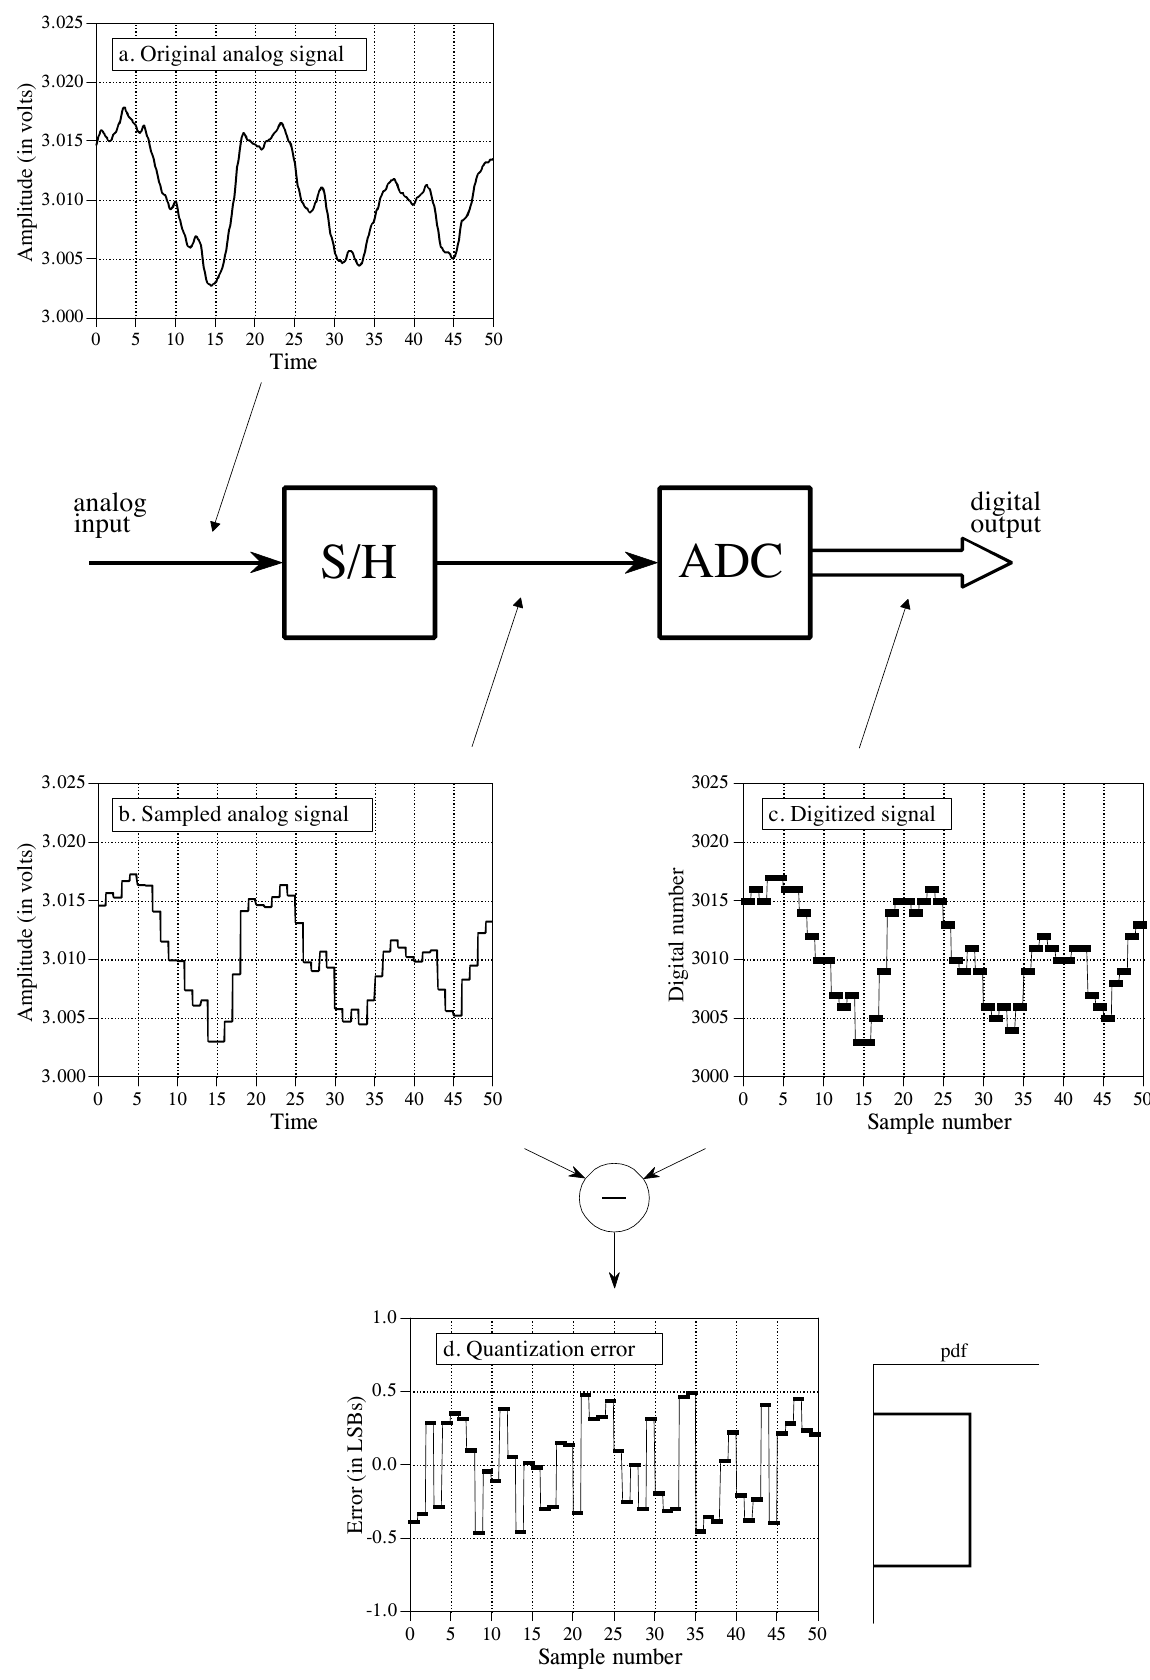
\includegraphics[width=0.958\linewidth,height=0.8\textheight,keepaspectratio]{assets/ch03/fig3-01.png}
\caption*{\textbf{图 3-1　说明数字化过程的波形。}
转换被拆成两个阶段，以便把采样的影响和量化的影响分开。第一阶段是采样保持(S/H)，只保留周期性采样那一刻信号的瞬时值。第二阶段由
ADC 把电压转换成最接近的整数。结果是数字化信号中每个采样都有最多 ±½ LSB
的误差，如 (d) 所示。因此，量化通常可以简单地建模为给信号加上噪声。 （a.
原始模拟信号(Original analog signal)；b. 采样后的模拟信号(Sampled analog
signal)；c.~数字化信号(Digitized signal)；d.~量化误差(Quantization
error)，右侧小图为其 pdf。框图：analog input = 模拟输入，digital output
= 数字输出。Amplitude (in volts) = 幅度（伏），Digital number =
数字值，Error (in LSBs) = 误差（以 LSB 为单位），Time = 时间，Sample
number = 采样序号。）}
\end{figure}

这个模型非常强大，因为量化产生的随机噪声只是简单地叠加到模拟信号中已有的噪声上。例如，设想一个最大幅度为
1.0 伏、随机噪声为 1.0 毫伏均方根值的模拟信号。把它数字化为 8 比特，1.0
伏变成数字 255，1.0 毫伏变成 0.255
LSB。上一章讲过，随机噪声信号叠加时，方差相加。也就是说，信号按平方和(quadrature)的方式相加：\(\sqrt{A^2 + B^2} = C\)。因此数字化信号上的总噪声为
\(\sqrt{0.255^2 + 0.29^2} = 0.386\) LSB，比模拟信号中原有的噪声增加了约
50\%。把同一个信号数字化为 12
比特，噪声几乎不会增加，量化也不会丢失任何东西。在决定一个系统需要多少比特时，问两个问题：(1)
模拟信号中原本已经有多少噪声？(2) 数字信号能容忍多少噪声？

这个量化模型什么时候不成立？只有当量化误差不能当作随机误差处理时。唯一常见的情况是：模拟信号在许多个连续采样中都保持在差不多同一个值，如图
3-2a 所示。即使模拟信号的变化可达 ±½
LSB，输出也会连续许多个采样卡在同一个数字上。这时量化误差不再是附加的随机噪声，而像是一种阈值效应，或者说一种古怪的失真。

抖动(dithering)是改善这类缓变信号数字化的常用技术。如图 3-2b
所示，给模拟信号加上少量随机噪声。本例中，加入的噪声呈正态分布，标准差为
2/3 LSB，峰峰值约为 3 LSB。图 (c)
显示了加入这种抖动噪声后数字化信号的变化。即使原始模拟信号的变化不到 ±½
LSB，加入的噪声也会让数字输出在相邻电平之间随机跳动。

要理解这为什么能改善情况，设想输入信号是恒定的模拟电压 3.0001
伏，正好位于数字电平 3000 和 3001
之间的十分之一处。不加抖动时，对这个信号取 10,000 个采样，会得到 10,000
个相同的数，全都是
3000。接着在加了少量抖动噪声的情况下重做这个思想实验。这 10,000
个值现在会在两个（或更多）电平之间摆动，大约 90\% 是 3000，10\% 是
3001。对全部 10,000 个值取平均，结果接近 3000.1。尽管单次测量有固有的 ±½
LSB
限制，大量采样的统计量却能做得好得多。这真是一种奇怪的情形：加入噪声反而提供了更多信息。

抖动电路可以做得相当精巧，比如用计算机生成随机数，再经过 DAC
产生要加入的噪声。数字化之后，计算机可以用浮点运算从数字信号中减去这些随机数。这种优雅的技术叫减性抖动(subtractive
dither)，但只用在最讲究的系统里。最简单的方法（虽然不一定总能做到）是直接利用模拟信号中已有的噪声来做抖动。

\begin{figure}[htbp]
\centering
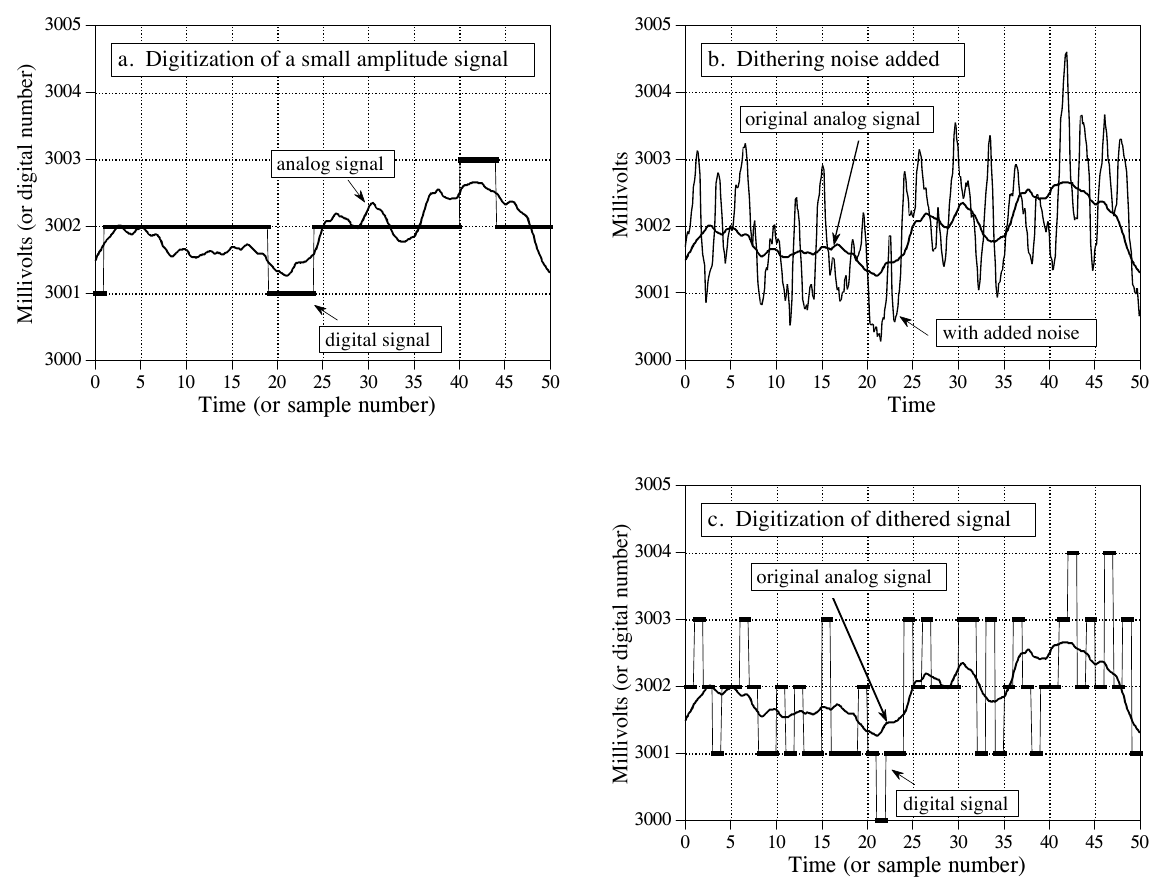
\includegraphics[width=0.958\linewidth,height=0.8\textheight,keepaspectratio]{assets/ch03/fig3-02.png}
\caption*{\textbf{图 3-2　抖动示意。} 图 (a) 显示，变化不到 ±½ LSB
的模拟信号在数字化时会卡在同一个量化电平上。抖动通过给模拟信号加入少量随机噪声来改善这种情况，如
(b) 所示。本例中，加入的噪声呈正态分布，标准差为 2/3 LSB。如 (c)
所示，加入的噪声使数字化信号在相邻量化电平之间跳动，从而提供了关于原始信号的更多信息。
（a. 小幅度信号的数字化(Digitization of a small amplitude signal)；b.
加入抖动噪声(Dithering noise added)；c.~抖动后信号的数字化(Digitization
of dithered signal)。original analog signal = 原始模拟信号，digital
signal = 数字信号，analog signal with added noise =
加了噪声的模拟信号，Millivolts (or digital number) =
毫伏（或数字值），Time (or sample number) = 时间（或采样序号）。）}
\end{figure}

\section{采样定理}

「正确采样」的定义非常简单。假设你以某种方式对一个连续信号做了采样。如果能从这些采样精确地重建出模拟信号，那么你的采样一定是正确的。即使采样数据看起来混乱或不完整，只要这个过程能逆转回去，关键信息就已经被捕获了。

图 3-3 展示了几个正弦波数字化前后的样子。连续的线代表进入 ADC
的模拟信号，方形标记是离开 ADC 的数字信号。在 (a)
中，模拟信号是恒定的直流值，即频率为零的余弦波。由于模拟信号在每两个采样之间都是直线，重建模拟信号所需的全部信息都包含在数字数据中。按照我们的定义，这是正确采样。

\begin{enumerate}
\def\labelenumi{(\alph{enumi})}
\setcounter{enumi}{1}
\tightlist
\item
  中的正弦波频率是采样率的 0.09 倍。比如，它可以代表以每秒 1000
  个采样的速率采样一个每秒 90
  周的正弦波。换一种说法，正弦波每个完整周期里取了 11.1
  个采样。这种情况比上一种复杂，因为不能只在数据点之间画直线来重建模拟信号。这些采样是否正确地代表了模拟信号？答案是肯定的，因为没有任何其他正弦波或正弦波组合会产生这样的采样模式（在下面列出的合理约束条件下）。这些采样只对应一个模拟信号，因此模拟信号可以被精确重建。这又是一个正确采样的例子。
\end{enumerate}

在 (c) 中，把正弦波的频率提高到采样率的 0.31
倍，情况变得更难了。这时每个正弦周期只有 3.2
个采样。采样如此稀疏，甚至看起来都不跟随模拟信号的大致走势。这些采样是否正确地代表了模拟波形？答案仍然是肯定的，理由完全相同：这些采样是模拟信号的唯一表示，重建连续波形所需的全部信息都包含在数字数据中。具体怎么做，本章后面会讨论。显然，这不能只靠在数据点之间画直线，必须更巧妙。尽管看起来很奇怪，按我们的定义，这是正确采样。

在 (d) 中，模拟频率被推到更高的采样率的 0.95 倍，每个正弦周期只有区区
1.05
个采样。这些采样是否正确地代表了数据？不，没有！这些采样代表的是另一个正弦波，而不是模拟信号中的那个。具体来说，原本频率为
0.95 的正弦波，在数字信号中冒充成了频率为 0.05
的正弦波。正弦波在采样过程中改变频率的这种现象叫混叠(aliasing)。就像罪犯可能用化名或假身份（alias）一样，正弦波冒用了一个不属于它的频率。由于数字数据不再唯一对应某个特定的模拟信号，无歧义的重建就不可能了。采样数据中没有任何东西表明原始模拟信号的频率是
0.95 而不是
0.05。正弦波彻底隐藏了自己的真实身份，一桩完美犯罪就此完成！按我们的定义，这是采样不正确的例子。

\begin{figure}[htbp]
\centering
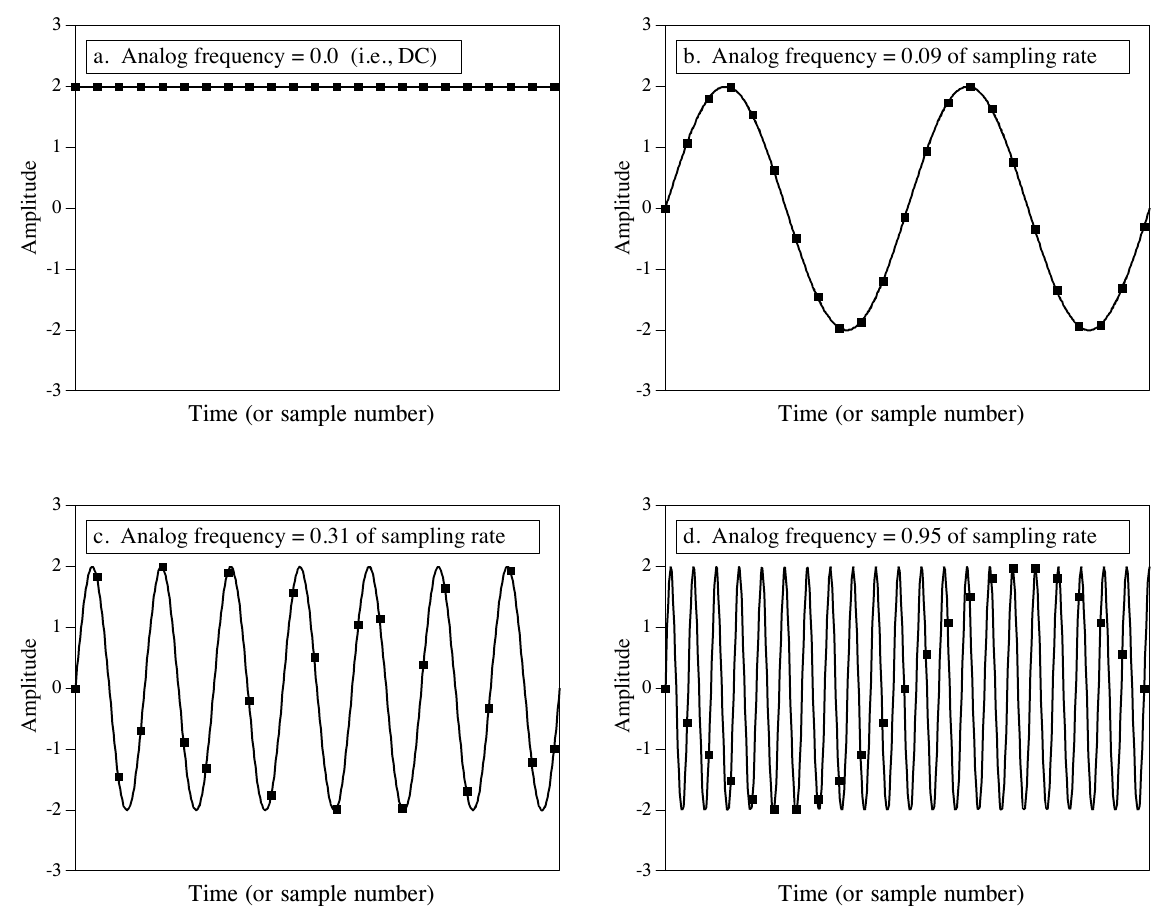
\includegraphics[width=0.967\linewidth,height=0.8\textheight,keepaspectratio]{assets/ch03/fig3-03.png}
\caption*{\textbf{图 3-3　正确采样与不正确采样的示意。}
如果采样包含了重建原始波形所需的全部信息，连续信号的采样就是正确的。图
(a)、(b)、(c) 展示了三个正弦波的正确采样。这一点当然不明显，因为 (c)
中的采样甚至看起来都没抓住波形的形状。尽管如此，这些连续信号中的每一个都和它的采样模式构成唯一的一一对应，这保证了重建可以进行。在
(d)
中，模拟正弦波的频率高于奈奎斯特频率（采样率的一半），导致混叠：采样数据的频率不同于连续信号的频率。由于混叠破坏了信息，原始信号无法从采样中重建。
（a. 模拟频率 = 0.0（即直流）；b. 模拟频率 = 采样率的 0.09
倍；c.~模拟频率 = 采样率的 0.31 倍；d.~模拟频率 = 采样率的 0.95
倍。Amplitude = 幅度，Time (or sample number) = 时间（或采样序号）。）}
\end{figure}

这一推理引出了 DSP 中的一个里程碑：采样定理(sampling
theorem)。它常被称为香农采样定理(Shannon sampling
theorem)或奈奎斯特采样定理(Nyquist sampling theorem)，以 20 世纪 40
年代发表相关论文的作者命名。采样定理指出：只有当连续信号不含高于采样率一半的频率成分时，它才能被正确采样。例如，每秒
2,000 个采样的采样率，要求模拟信号由低于每秒 1000
周的频率组成。如果信号中存在高于这个上限的频率，它们就会被混叠到每秒 0
到 1000 周之间的频率上，和那里原本合法存在的信息混在一起。

讨论采样定理时，有两个术语用得很广：奈奎斯特频率(Nyquist
frequency)和奈奎斯特速率(Nyquist
rate)。遗憾的是，它们的含义并不统一。为了说明这一点，考虑一个由直流到 3
kHz 之间的频率组成的模拟信号。要正确地数字化这个信号，采样率必须达到每秒
6,000 个采样（6 kHz）或更高。假设我们选择以每秒 8,000 个采样（8
kHz）采样，这样直流到 4 kHz
之间的频率都能被正确表示。这时有四个重要的频率：(1) 信号中的最高频率 3
kHz；(2) 它的两倍 6 kHz；(3) 采样率 8 kHz；(4) 采样率的一半 4
kHz。这四个中哪个是奈奎斯特频率，哪个是奈奎斯特速率？看你问谁了！所有可能的组合都有人用。好在大多数作者都会仔细说明自己怎么用这些术语。本书中，两者都指采样率的一半。

图 3-4
展示了混叠过程中频率是怎样改变的。要记住的关键一点是：数字信号不可能包含高于采样率一半（即奈奎斯特频率/速率）的频率。当连续波的频率低于奈奎斯特速率时，采样数据的频率与之相符。但当连续信号的频率高于奈奎斯特速率时，混叠会把这个频率变成采样数据能表示的某个频率。如图
3-4 中的锯齿线所示，高于奈奎斯特速率的每个连续频率，都对应 0
到采样率一半之间的某个数字频率。如果这个较低的频率上恰好已经有一个正弦波，混叠过来的信号就会加到它上面，造成信息损失。混叠是双重诅咒：较高频率和较低频率的信息都可能丢失。假设给你一个包含采样率
0.2
倍频率的数字信号。如果这个信号是正确采样得到的，原始模拟信号的频率一定是
0.2。如果采样时发生了混叠，数字频率 0.2
可能来自模拟信号中无穷多个频率中的任何一个：0.2、0.8、1.2、1.8、2.2、\ldots{}

混叠在采样时能改变频率，也能改变相位(phase)。例如，回头看图 3-3d
中混叠后的信号。混叠后的数字信号相对原始模拟信号是反相的：一个是正弦波，另一个是负的正弦波。换句话说，混叠改变了频率，还引入了
180° 的相移。可能的相移只有两种：0°（无相移）和 180°（反相）。模拟频率在
0 到 0.5、1.0 到 1.5、2.0 到 2.5 等范围内时，相移为零；在 0.5 到
1.0、1.5 到 2.0、2.5 到 3.0 等范围内时，相位反转。

现在我们深入更细致地分析采样以及混叠是怎样发生的。总体目标是理解：信号从连续形式转换成离散形式时，信息发生了什么。问题在于，这两样东西非常不同：一个是连续波形，另一个是一组数。这种「苹果比橘子」的比较让分析变得非常困难。解决办法是引入一个叫冲激串(impulse
train)的理论概念。

图 3-5a 是一个模拟信号的例子。图 (c)
是用冲激串对它采样的结果。冲激串是一个连续信号，由一系列窄尖峰（冲激(impulses)）组成，这些尖峰在采样时刻与原始信号相等。每个冲激都无限窄，这个概念将在第
13
章讨论。在采样时刻之间，波形的值为零。记住，冲激串是一个理论概念，而不是能在电子电路中真实存在的波形。由于原始模拟信号和冲激串都是连续波形，我们就能在两者之间做「苹果比苹果」的比较了。

\begin{figure}[htbp]
\centering
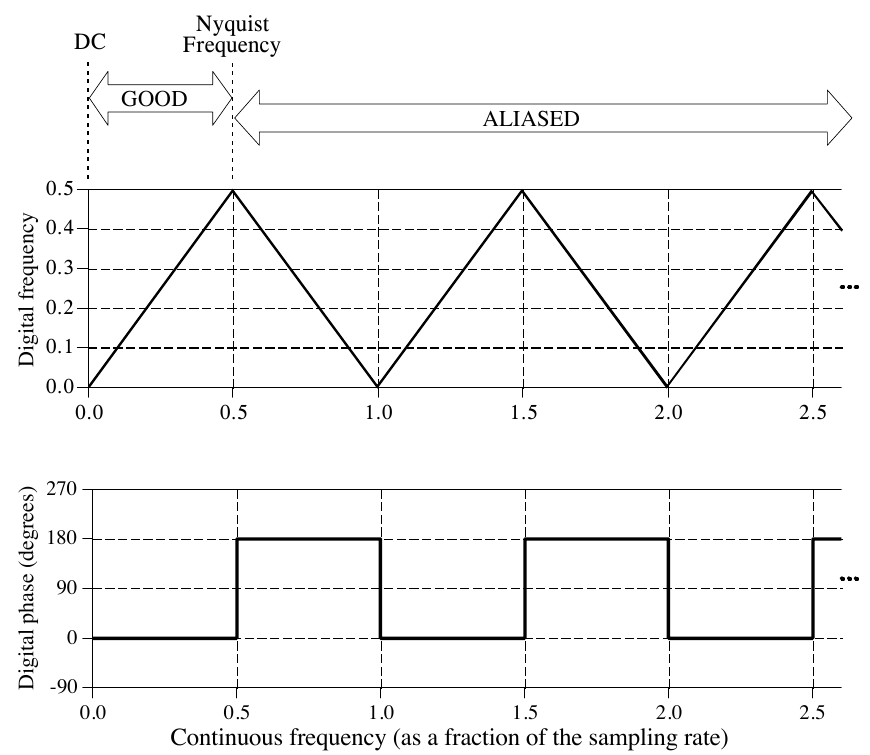
\includegraphics[width=0.725\linewidth,height=0.8\textheight,keepaspectratio]{assets/ch03/fig3-04.png}
\caption*{\textbf{图 3-4　采样时模拟频率到数字频率的转换。}
频率低于采样率一半的连续信号，直接转换成对应的数字频率。高于采样率一半时发生混叠，频率在数字数据中被错误表示。混叠总是把较高的频率变成
0 到 0.5 之间某个较低的频率。此外，混叠还可能把信号的相位改变 180 度。
（上图：Digital frequency = 数字频率，DC = 直流，Nyquist Frequency =
奈奎斯特频率，GOOD = 正确，ALIASED = 混叠。下图：Digital phase (degrees)
= 数字相位（度）。横轴：Continuous frequency (as a fraction of the
sampling rate) = 连续频率（以采样率的倍数表示）。）}
\end{figure}

现在需要研究冲激串和离散信号（一组数）之间的关系。这个很简单：就信息含量而言，两者完全相同。知道其中一个，算出另一个是小事一桩。可以把它们看作横跨模拟世界和数字世界的一座桥的两端。这意味着，只要我们弄懂了把图
3-5a 的波形变成图 3-5c 的波形会带来什么后果，总体目标就达成了。

图 3-5 左栏是三个连续波形，右栏是这些信号对应的频谱(frequency
spectra)。从你的电子学知识来看，这应该是个熟悉的概念：每个波形都可以看作由幅度和频率各异的正弦波组成。后面的章节会详细讨论频域。（等你更熟悉频谱之后，可能想回头再看看这段讨论。）

图 (a) 是我们想要采样的模拟信号。从 (b) 中它的频谱可以看出，它只由 0
到大约 0.33 \(f_s\) 之间的频率成分组成，\(f_s\)
是我们打算使用的采样频率。比如，这可能是一个已滤除了 3.3 kHz
以上所有频率的语音信号。相应地，\(f_s\) 就是 10 kHz（每秒 10,000
个采样），也就是我们打算用的采样率。

用冲激串对 (a) 中的信号采样，得到 (c) 所示的信号，以及 (d)
所示的频谱。这个频谱是原始信号频谱的复制：采样频率的每个整数倍
\(f_s\)、\(2f_s\)、\(3f_s\)、\(4f_s\)
等处，都得到了原始频谱的一份拷贝和一份左右翻转的拷贝。拷贝叫上边带(upper
sideband)，翻转的拷贝叫下边带(lower
sideband)。采样产生了新的频率。这是正确采样吗？答案是肯定的，因为只要去掉
½\(f_s\) 以上的所有频率，(c) 中的信号就能变回 (a)
中的信号。也就是说，一个模拟低通滤波器(low-pass filter)可以把冲激串 (b)
变回原始的模拟信号 (a)。

如果你已经熟悉 DSP
的基础，这里有一个更技术性的解释，说明为什么会出现这种频谱复制。（如果你刚接触
DSP，可以跳过这一段。）在时域中，采样是通过把原始信号乘以一个由单位幅度尖峰组成的冲激串来实现的。这个单位幅度冲激串的频谱，也是一个单位幅度冲激串，尖峰出现在采样频率的整数倍
\(f_s\)、\(2f_s\)、\(3f_s\)、\(4f_s\)
等处。两个时域信号相乘时，它们的频谱做卷积(convolve)。结果是原始频谱被复制到冲激串频谱中每个尖峰的位置上。把原始信号看作同时由正频率和负频率组成，就分别解释了上边带和下边带。这和第
10 章讨论的幅度调制(amplitude modulation)是一回事。

图 (e) 是一个采样不正确的例子，原因是采样率太低。模拟信号仍然包含高达
3.3 kHz 的频率，但采样率降到了 5 kHz。注意横轴上
\(f_s\)、\(2f_s\)、\(3f_s\) \ldots{} 在 (f) 中比在 (d) 中排得更密。频谱
(f) 揭示了问题所在：复制出来的那部分频谱侵入了 0
到采样频率一半之间的频带。虽然 (f)
把这些重叠的频率画得还能分辨，但实际上它们会加在一起，形成一团乱麻。由于没有办法把重叠的频率分开，信息就丢失了，原始信号无法重建。当模拟信号包含高于采样率一半的频率时，就会发生这种重叠。也就是说，我们证明了采样定理。

\begin{figure}[htbp]
\centering
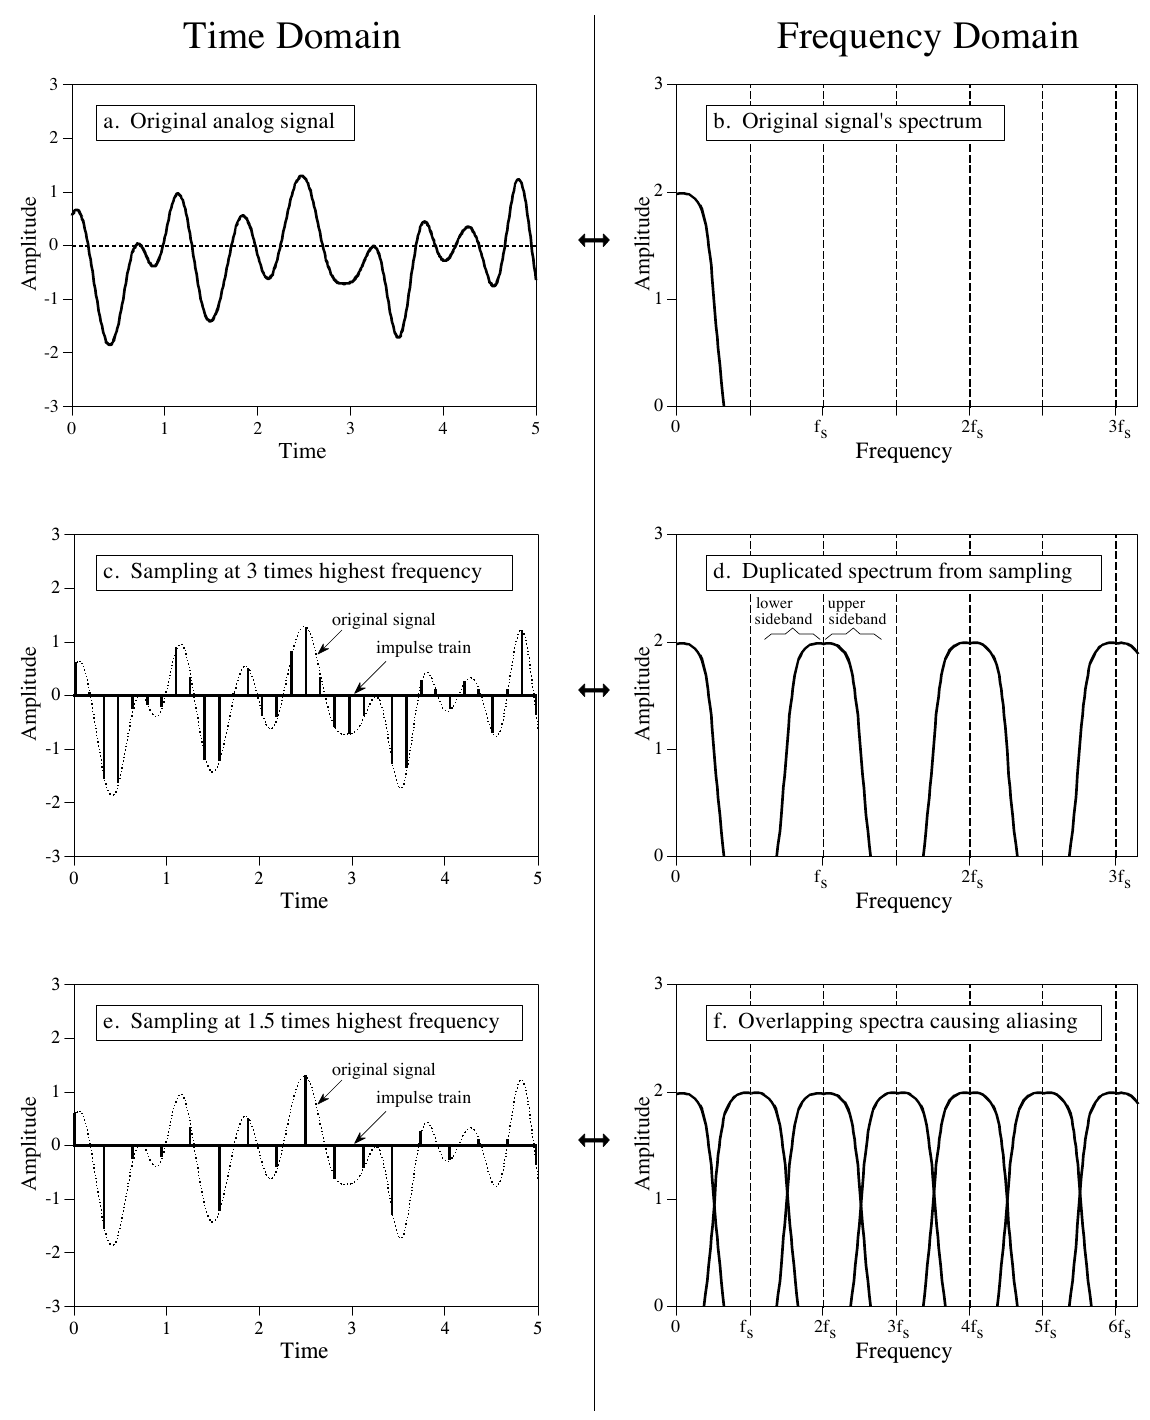
\includegraphics[width=0.958\linewidth,height=0.8\textheight,keepaspectratio]{assets/ch03/fig3-05.png}
\caption*{\textbf{图 3-5　时域和频域中的采样定理。} 图 (a) 和 (b) 是一个由 0 到
0.33 倍采样频率 \(f_s\) 之间的频率成分组成的模拟信号。在 (c)
中，把模拟信号转换成冲激串，以此对它采样。在频域 (d)
中，这使频谱被复制成无穷多个上边带和下边带。由于 (b) 中的原始频率在 (d)
中没有失真地保留着，所以采样是正确的。相比之下，(e)
中的模拟信号（其最高频率）达到采样频率的 0.66
倍，超过了奈奎斯特速率。这导致了混叠，表现为 (f) 中的边带相互重叠。
（左栏 Time Domain = 时域，右栏 Frequency Domain = 频域。a.
原始模拟信号；b. 原始信号的频谱；c.~以最高频率的 3 倍采样（original
signal = 原始信号，impulse train =
冲激串）；d.~采样造成的频谱复制（lower sideband = 下边带，upper sideband
= 上边带）；e. 以最高频率的 1.5 倍采样；f.~频谱重叠导致混叠。Amplitude =
幅度，Time = 时间，Frequency = 频率。）}
\end{figure}

\section{数模转换}

理论上，最简单的数模转换方法是从存储器中取出采样，把它们转换成冲激串。如图
3-6a 所示，对应的频谱见
(b)。正如刚才所说，让这个冲激串通过一个截止频率等于采样率一半的低通滤波器，就能完美地重建原始模拟信号。换句话说，在奈奎斯特频率（采样率的一半）以下，原始信号和冲激串的频谱完全相同。在更高的频率上，冲激串包含这些信息的复制品，而原始模拟信号什么都没有（假设没有发生混叠）。

这种方法虽然在数学上很纯粹，但在电子电路中很难产生所需的窄脉冲。为了绕开这个问题，几乎所有
DAC
都是把上一个值保持住，直到收到下一个采样为止。这叫零阶保持(zeroth-order
hold)，相当于 ADC 中采样保持在 DAC
这一端的对应物。（一阶保持是在点之间连直线，二阶保持用抛物线，依此类推。）零阶保持产生
(c) 中那样的阶梯状外观。

在频域中，零阶保持使冲激串的频谱乘上了 (d) 中那条深色曲线，其公式为：

\textbf{公式 3-1　零阶保持造成的高频幅度衰减。} 这条曲线画在图 3-6d
中。\(f_s\) 表示采样频率。当 f = 0 时，H(f) = 1。

\[
H(f) = \left|\,\frac{\sin(\pi f / f_s)}{\pi f / f_s}\,\right|
\]

它的一般形式是 \(\sin(\pi x)/(\pi x)\)，叫 sinc 函数，记作 sinc(x)。sinc
函数在 DSP
中非常常见，后面的章节会更详细地讨论。如果你已有这方面的背景，可以把零阶保持理解为冲激串与一个宽度等于采样周期的矩形脉冲做卷积。这使频域乘上了矩形脉冲的傅里叶变换(Fourier
transform)，也就是 sinc 函数。在图 (d)
中，浅色线是冲激串的频谱（「正确的」频谱），深色线是
sinc。零阶保持信号的频谱等于这两条曲线的乘积。

用来把零阶保持信号 (c) 转换成重建信号 (f)
的模拟滤波器，需要做两件事：(1) 去掉采样率一半以上的所有频率；(2)
按零阶保持效应的倒数，即
1/sinc(x)，提升各个频率。这相当于在采样频率一半处放大约 36\%。图 (e)
是这个模拟滤波器的理想频率响应。

\begin{figure}[htbp]
\centering
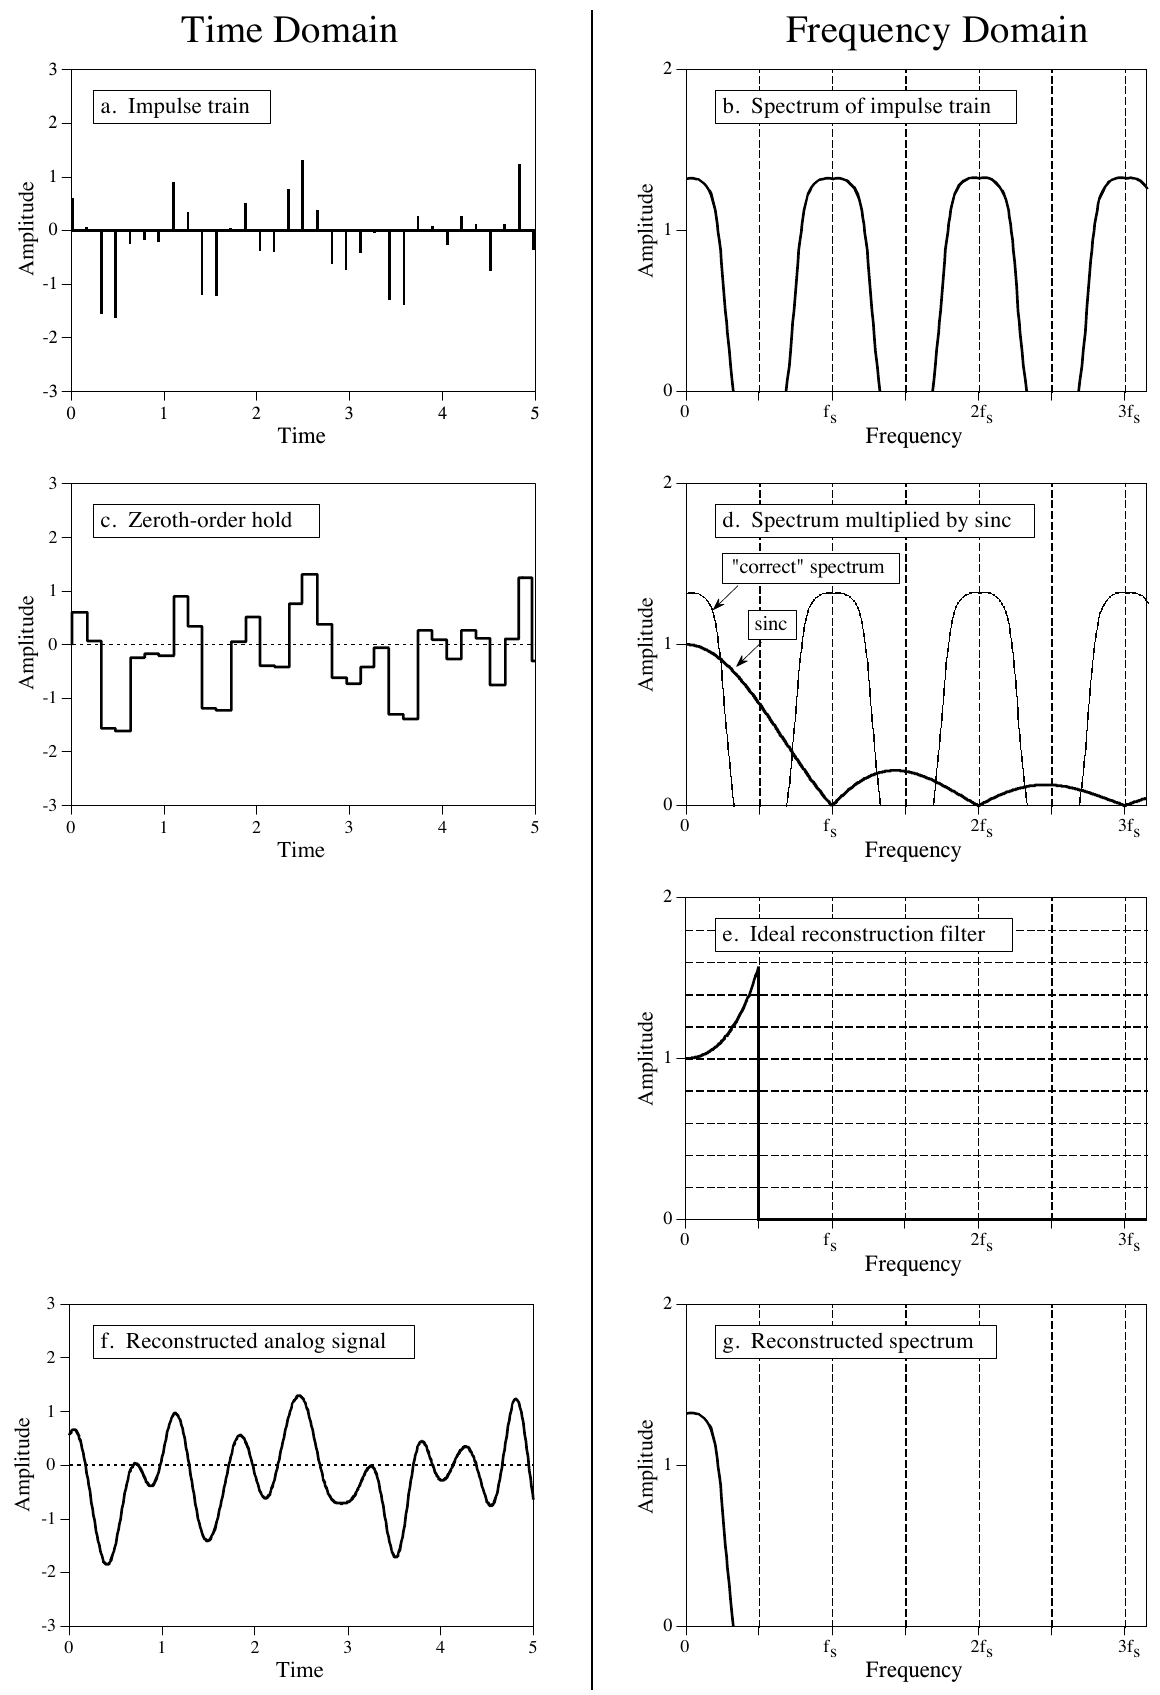
\includegraphics[width=0.967\linewidth,height=0.8\textheight,keepaspectratio]{assets/ch03/fig3-06.png}
\caption*{\textbf{图 3-6　数模转换的分析。} 在 (a)
中，数字数据被转换成冲激串，其频谱见
(b)。用一个电子低通滤波器去掉采样率一半以上的频率，就能把它变成重建信号
(f)［比较 (b) 和 (g)］。然而，大多数电子 DAC 产生的是零阶保持波形
(c)，而不是冲激串。零阶保持的频谱等于冲激串的频谱乘以 (d) 中所示的 sinc
函数。要把零阶保持信号变成重建信号，模拟滤波器必须去掉奈奎斯特速率以上的所有频率，并校正
sinc 的影响，如 (e) 所示。 （a. 冲激串(Impulse train)；b.
冲激串的频谱；c.~零阶保持(Zeroth-order hold)；d.~频谱乘以
sinc（``correct'' spectrum = 「正确的」频谱）；e. 理想重建滤波器(Ideal
reconstruction filter)；f.~重建的模拟信号；g. 重建的频谱。Amplitude =
幅度，Time = 时间，Frequency = 频率。）}
\end{figure}

这种 1/sinc(x) 的频率提升有四种处理方式：(1) 忽略它，接受后果；(2)
设计一个包含 1/sinc(x) 响应的模拟滤波器；(3)
使用本章后面介绍的一种巧妙的多速率(multirate)技术；(4) 在 DAC
之前用软件做校正（见第 24 章）。

在结束关于采样的这一节之前，我们需要破除一个关于模拟信号与数字信号的常见迷思。正如本章所示，数字信号携带的信息量受两方面的限制：第一，每个采样的比特数限制了因变量的分辨率。也就是说，信号幅度的微小变化可能淹没在量化噪声中。第二，采样率限制了自变量的分辨率，即模拟信号中间隔很近的事件可能在两个采样之间丢失。这只是「采样率一半以上的频率会丢失」的另一种说法。

迷思是这样的：「既然模拟信号使用连续的参数，它们在自变量和因变量上都有无限好的分辨率。」不对！模拟信号受到和数字信号同样两个问题的限制：噪声和带宽(bandwidth，信号中允许的最高频率)。模拟信号中的噪声限制了波形幅度的测量，就像数字信号中的量化噪声一样。同样，在模拟信号中分辨间隔很近的事件的能力，取决于波形中允许的最高频率。为了理解这一点，设想一个包含两个间隔很近的脉冲的模拟信号。如果让这个信号通过一个低通滤波器（去掉高频），两个脉冲就会模糊成一团。例如，由直流到
10 kHz 之间的频率构成的模拟信号，和以 20 kHz
采样的数字信号有完全相同的分辨率。必然如此，因为采样定理保证了两者包含相同的信息。

\section{用于数据转换的模拟滤波器}

图 3-7 是采样定理所要求的 DSP
系统框图。输入信号在进入模数转换器之前，先经过一个电子低通滤波器，去掉奈奎斯特频率（采样率的一半）以上的所有频率。这是为了防止采样时发生混叠，因此相应地称为抗混叠滤波器(antialias
filter)。在另一端，数字化信号经过数模转换器和另一个设在奈奎斯特频率的低通滤波器。这个输出滤波器叫重建滤波器(reconstruction
filter)，可能包含前面讲的零阶保持频率提升。遗憾的是，这个简单模型有一个严重问题：电子滤波器的局限，可能和它们试图防止的问题一样糟糕。

\begin{figure}[htbp]
\centering
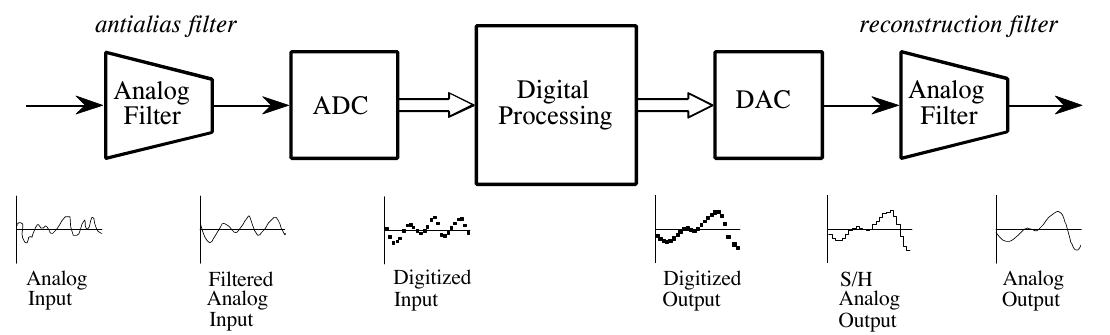
\includegraphics[width=0.925\linewidth,height=0.8\textheight,keepaspectratio]{assets/ch03/fig3-07.png}
\caption*{\textbf{图 3-7　为满足采样定理而使用的模拟电子滤波器。} 放在 ADC
之前的电子滤波器叫抗混叠滤波器，用来去掉采样时会发生混叠的、高于采样率一半的频率成分。放在
DAC
之后的电子滤波器叫重建滤波器，它同样去掉奈奎斯特速率以上的频率，并可能包含对零阶保持的校正。
（antialias filter = 抗混叠滤波器，reconstruction filter =
重建滤波器，Analog Filter = 模拟滤波器，Digital Processing =
数字处理。信号依次为：Analog Input = 模拟输入 \dspsym{→} Filtered Analog
Input = 滤波后的模拟输入 \dspsym{→} Digitized Input = 数字化输入
\dspsym{→} Digitized Output = 数字化输出 \dspsym{→} S/H Analog Output =
采样保持后的模拟输出 \dspsym{→} Analog Output = 模拟输出。）}
\end{figure}

如果你主要关心软件，可能会觉得不需要读这一节。错！即使你发誓永远不碰示波器，理解模拟滤波器的特性对做好
DSP
也很重要。第一，你遇到的每个数字化信号的特性，都取决于采集它时用了哪种抗混叠滤波器。不了解抗混叠滤波器的性质，就无法了解数字信号的性质。第二，DSP
的未来是用软件取代硬件。例如，本章后面介绍的多速率技术，就用巧妙的软件技巧减少了对抗混叠滤波器和重建滤波器的需求。不懂硬件，就没法设计软件来取代它。第三，DSP
的很大一部分和数字滤波器设计有关。常用的策略是从一个等效的模拟滤波器出发，把它转换成软件。后面的章节假定你对模拟滤波器技术有基本的了解。

常用的模拟滤波器有三种：切比雪夫(Chebyshev)、巴特沃斯(Butterworth)和贝塞尔(Bessel，也叫汤普森(Thompson)滤波器)。每一种都是为优化某一项不同的性能参数而设计的。每种滤波器的复杂度都可以通过选择极点(poles)和零点(zeros)的个数来调节，这两个数学术语后面的章节会讨论。滤波器的极点越多，需要的电子元件就越多，性能也越好。这些名字描述的是滤波器的作用，而不是电阻和电容的某种特定排列。例如，一个
6 极点贝塞尔滤波器可以用许多不同类型的电路实现，它们的整体特性都相同。就
DSP
而言，这些滤波器的特性比它们怎样搭建更重要。尽管如此，我们还是先简短介绍一下这些滤波器的电子设计，以提供一个整体框架。

图 3-8 是模拟滤波器设计中的一个常用基本单元：改进型 Sallen-Key
电路(modified Sallen-Key circuit)，以 20 世纪 50
年代描述这一技术的论文作者命名。图中所示的电路是一个 2
极点低通滤波器，可以配置成三种基本类型中的任意一种。表 3-1
提供了选择合适电阻和电容所需的信息。例如，要设计一个 1 kHz、2
极点的巴特沃斯滤波器，表 3-1 给出参数：k1 = 0.1592，k2 = 0.586。随意选取
R1 = 10K 和 C = 0.01 µF（运放电路的常用值），就能算出 R 和 Rf 分别为
15.95K 和 5.86K。把后两个值取整到最接近的 1\% 标准电阻，得到 R =
15.8K，Rf = 5.90K。所有元件的精度都应在 1\% 或更好。

\begin{figure}[htbp]
\centering
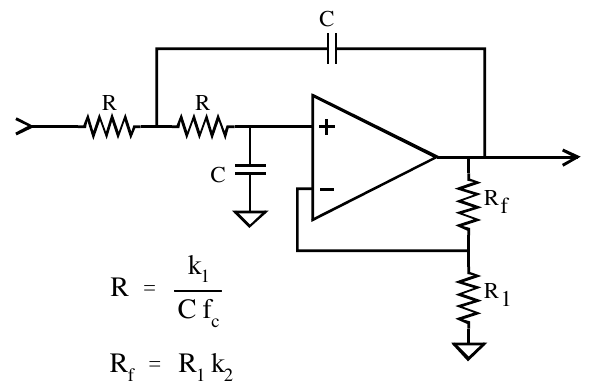
\includegraphics[width=0.496\linewidth,height=0.8\textheight,keepaspectratio]{assets/ch03/fig3-08.png}
\caption*{\textbf{图 3-8　改进型 Sallen-Key 电路，有源滤波器设计的基本单元。}
图示电路实现一个 2
极点低通滤波器。级联多级可以构成更高阶（更多极点）的滤波器。从表 3-1
查出 k1 和 k2，随意选取 R1 和 C（可以试试 10K 和 0.01
µF），再用图中的公式算出 R 和 Rf。参数 \(f_c\)
是滤波器的截止频率，单位为赫兹。}
\end{figure}

图中的两个公式：

\[
R = \frac{k_1}{C\,f_c}, \qquad R_f = R_1\,k_2
\]

\textbf{表 3-1　设计贝塞尔、巴特沃斯和切比雪夫（6\%
纹波）滤波器的参数。}

\begingroup\scriptsize\setlength{\tabcolsep}{3pt}

{\def\LTcaptype{none} % do not increment counter
\begin{longtable}[]{@{}
  >{\raggedright\arraybackslash}p{(\linewidth - 14\tabcolsep) * \real{0.1000}}
  >{\raggedright\arraybackslash}p{(\linewidth - 14\tabcolsep) * \real{0.1000}}
  >{\raggedleft\arraybackslash}p{(\linewidth - 14\tabcolsep) * \real{0.1333}}
  >{\raggedleft\arraybackslash}p{(\linewidth - 14\tabcolsep) * \real{0.1333}}
  >{\raggedleft\arraybackslash}p{(\linewidth - 14\tabcolsep) * \real{0.1333}}
  >{\raggedleft\arraybackslash}p{(\linewidth - 14\tabcolsep) * \real{0.1333}}
  >{\raggedleft\arraybackslash}p{(\linewidth - 14\tabcolsep) * \real{0.1333}}
  >{\raggedleft\arraybackslash}p{(\linewidth - 14\tabcolsep) * \real{0.1333}}@{}}
\toprule\noalign{}
\begin{minipage}[b]{\linewidth}\raggedright
极点数
\end{minipage} & \begin{minipage}[b]{\linewidth}\raggedright
级
\end{minipage} & \begin{minipage}[b]{\linewidth}\raggedleft
贝塞尔 k1
\end{minipage} & \begin{minipage}[b]{\linewidth}\raggedleft
贝塞尔 k2
\end{minipage} & \begin{minipage}[b]{\linewidth}\raggedleft
巴特沃斯 k1
\end{minipage} & \begin{minipage}[b]{\linewidth}\raggedleft
巴特沃斯 k2
\end{minipage} & \begin{minipage}[b]{\linewidth}\raggedleft
切比雪夫 k1
\end{minipage} & \begin{minipage}[b]{\linewidth}\raggedleft
切比雪夫 k2
\end{minipage} \\
\midrule\noalign{}
\endhead
\bottomrule\noalign{}
\endlastfoot
2 & 第 1 级 & 0.1251 & 0.268 & 0.1592 & 0.586 & 0.1293 & 0.842 \\
4 & 第 1 级 & 0.1111 & 0.084 & 0.1592 & 0.152 & 0.2666 & 0.582 \\
& 第 2 级 & 0.0991 & 0.759 & 0.1592 & 1.235 & 0.1544 & 1.660 \\
6 & 第 1 级 & 0.0990 & 0.040 & 0.1592 & 0.068 & 0.4019 & 0.537 \\
& 第 2 级 & 0.0941 & 0.364 & 0.1592 & 0.586 & 0.2072 & 1.448 \\
& 第 3 级 & 0.0834 & 1.023 & 0.1592 & 1.483 & 0.1574 & 1.846 \\
8 & 第 1 级 & 0.0894 & 0.024 & 0.1592 & 0.038 & 0.5359 & 0.522 \\
& 第 2 级 & 0.0867 & 0.213 & 0.1592 & 0.337 & 0.2657 & 1.379 \\
& 第 3 级 & 0.0814 & 0.593 & 0.1592 & 0.889 & 0.1848 & 1.711 \\
& 第 4 级 & 0.0726 & 1.184 & 0.1592 & 1.610 & 0.1582 & 1.913 \\
\end{longtable}
}

\endgroup

所用的具体运放(op
amp)型号并不关键，只要它的单位增益频率比滤波器的截止频率高 30 到 100
倍以上即可。只要滤波器的截止频率低于约 100 kHz，这个要求很容易满足。

4、6、8 极点的滤波器，分别由 2、3、4
个这样的电路级联(cascade)而成。例如，图 3-9 是一个 6
极点贝塞尔滤波器的原理图，它由表 3-1 中的三级构成。每一级的 k1 和 k2
参数都不同，R 和 Rf 也随之不同。

\begin{figure}[htbp]
\centering
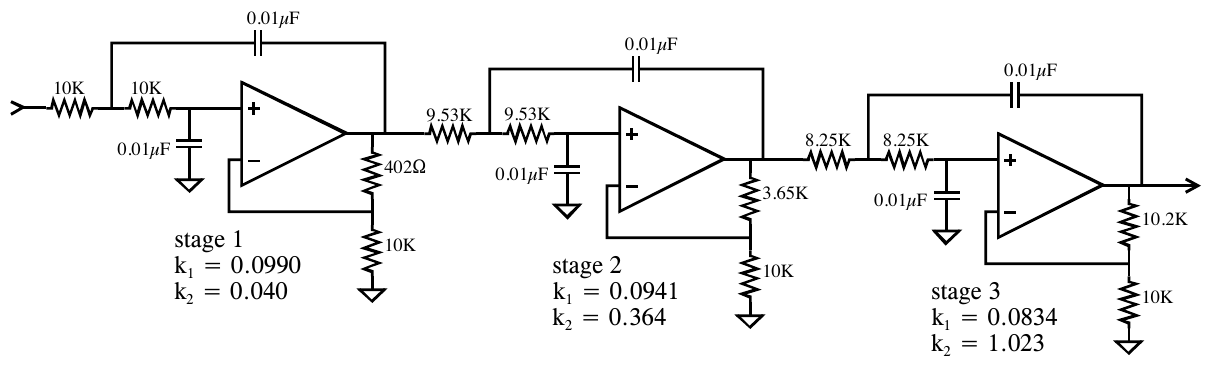
\includegraphics[width=1.000\linewidth,height=0.8\textheight,keepaspectratio]{assets/ch03/fig3-09.png}
\caption*{\textbf{图 3-9　由三个 Sallen-Key 电路级联构成的 6 极点贝塞尔滤波器。}
这是一个截止频率为 1 kHz 的低通滤波器。 （stage 1/2/3 = 第 1/2/3
级，各级标出了所用的 k1、k2。）}
\end{figure}

需要高通滤波器(high-pass filter)？只要把电路中的 R 和 C 元件对调即可（Rf
和 R1 保持不动）。

这类电路在小批量制造和研发应用中非常常见；但真正的量产要求把滤波器做成集成电路(integrated
circuit)。问题在于，直接在硅片上做电阻很难。答案是开关电容滤波器。图
3-10 把它和一个简单的 RC
网络作比较，以说明它的工作原理。如果把阶跃函数(step function)送入 RC
低通滤波器，输出会按指数规律上升，直到与输入相等。电容上的电压不会瞬间改变，因为电阻限制了电荷的流动。

开关电容滤波器的做法，是用两个电容和一个电子开关取代基本的电阻-电容网络。新加入的电容比原有的电容小得多，比如只有它的
1\%。开关以很高的频率（通常比滤波器的截止频率快 100
倍）交替地把小电容接到输入端和输出端。开关接到输入端时，小电容迅速充电到输入端当前的电压。开关接到输出端时，小电容上的电荷转移到大电容上。在电阻中，电荷转移的速率由阻值决定；在开关电容电路中，电荷转移的速率由小电容的容值和开关频率决定。这带来了开关电容滤波器一个非常有用的特性：滤波器的截止频率与驱动开关的时钟频率成正比。这使开关电容滤波器非常适合以多种采样率工作的数据采集系统。这些器件很好用：花十块钱，就能在一个
8 引脚的集成电路里得到 8 极点滤波器的性能。

\begin{figure}[htbp]
\centering
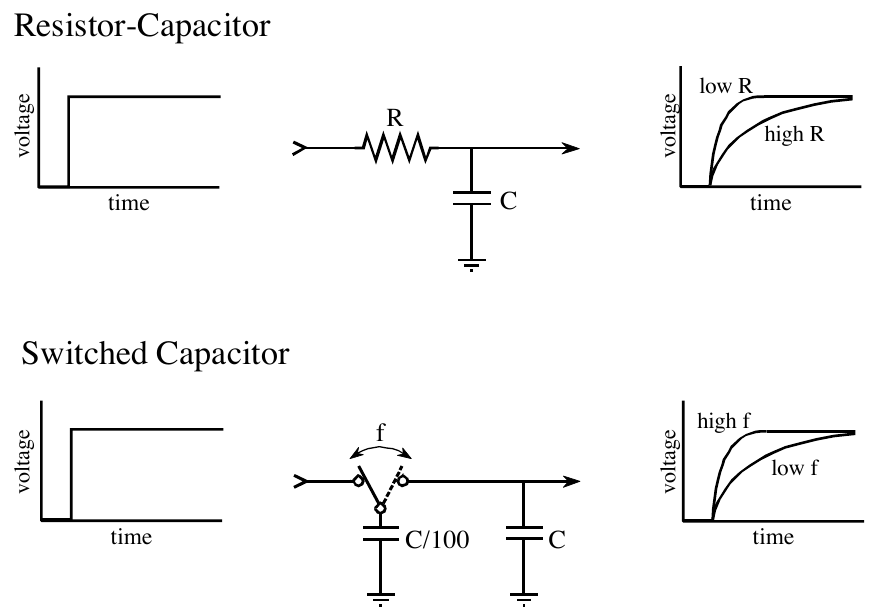
\includegraphics[width=0.733\linewidth,height=0.8\textheight,keepaspectratio]{assets/ch03/fig3-10.png}
\caption*{\textbf{图 3-10　开关电容滤波器的工作原理。}
开关电容滤波器用开关和电容来模拟电阻。如等效的阶跃响应所示，两个电容加一个开关可以起到和电阻-电容网络相同的作用。
（上：Resistor-Capacitor = 电阻-电容网络，low R / high R =
小电阻/大电阻；下：Switched Capacitor = 开关电容，high f / low f =
高/低开关频率，小电容为 C/100。voltage = 电压，time = 时间。）}
\end{figure}

现在讲重点：三种经典滤波器的特性。我们要考察的第一个性能参数是截止的陡峭程度。低通滤波器的设计目标是阻断截止频率以上的所有频率（阻带(stopband)），同时让截止频率以下的所有频率通过（通带(passband)）。图
3-11
以对数（dB）刻度展示了这三种滤波器的频率响应。图中的滤波器截止频率都是 1
赫兹，但可以直接按比例换算到你需要的任何截止频率。这些滤波器表现如何？切比雪夫显然最好，巴特沃斯差一些，贝塞尔简直糟透了！你大概已经猜到了，这正是切比雪夫的设计目标：尽可能快地滚降(roll-off，幅度下降)。

遗憾的是，即使是 8
极点切比雪夫滤波器，用作抗混叠滤波器也不如你希望的那样好。例如，设想一个以每秒
10,000 个采样采样的 12 比特系统。采样定理规定，5 kHz
以上的任何频率都会发生混叠，这是你想避免的。稍加估算，你决定 5 kHz
以上的所有频率在幅度上都必须衰减到
1/100，以保证任何混叠频率的幅度都小于百分之一。查看图
3-11c，你会发现截止频率为 1 赫兹的 8 极点切比雪夫滤波器，要到大约 1.35
赫兹才能达到 100
倍的衰减(attenuation，信号减小)。换算到这个例子，滤波器的截止频率必须设在
3.7 kHz，才能让 5 kHz 以上的一切都达到所需的衰减。这导致 3.7 kHz 到 5
kHz 之间的频带浪费在模拟滤波器不够陡的滚降上。

一个微妙之处：尽管 12 比特有 4096 级，本例中 100
倍的衰减很可能也够了。由图 3-4，5100 赫兹会混叠到 4900 赫兹，6000
赫兹会混叠到 4000 赫兹，依此类推。你并不在乎 5000 到 6300
赫兹之间信号的幅度，因为它们混叠到的是 3700 到 5000
赫兹之间那段不可用的区域。一个频率要混叠进滤波器的通带（0 到 3.7
kHz），它必须高于 6300 赫兹，即 3700 赫兹截止频率的 1.7 倍。如图 3-11c
所示，8 极点切比雪夫滤波器在截止频率 1.7 倍处的衰减约为
1300，比我们分析开始时设定的 100
充裕得多。这个故事的寓意是：在大多数系统中，大约 0.4 到 0.5
倍采样频率之间的频带，是一片充斥着滤波器滚降和混叠信号的不可用荒地。这是模拟滤波器局限的直接结果。

完美低通滤波器的频率响应在整个通带内是平坦的。在图 3-11
中，所有滤波器在这方面看起来都很好，但这只是因为纵轴用的是对数刻度。把图换成线性纵轴刻度，情况就不一样了，如图
3-12 所示。这时就能看到切比雪夫滤波器的通带纹波(passband
ripple，通过频率的幅度呈波浪状变化)。事实上，切比雪夫滤波器正是靠允许这种通带纹波，才获得了出色的滚降。滤波器允许的通带纹波越大，滚降就能越快。用表
3-1 设计的所有切比雪夫滤波器，通带纹波都约为 6\%（0.5
dB），这是一个不错的折中，也是常见的选择。一种类似的设计------椭圆滤波器(elliptic
filter)------在通带和阻带中都允许纹波。椭圆滤波器虽然更难设计，但能在滚降和通带纹波之间取得更好的平衡。

\begin{figure}[htbp]
\centering
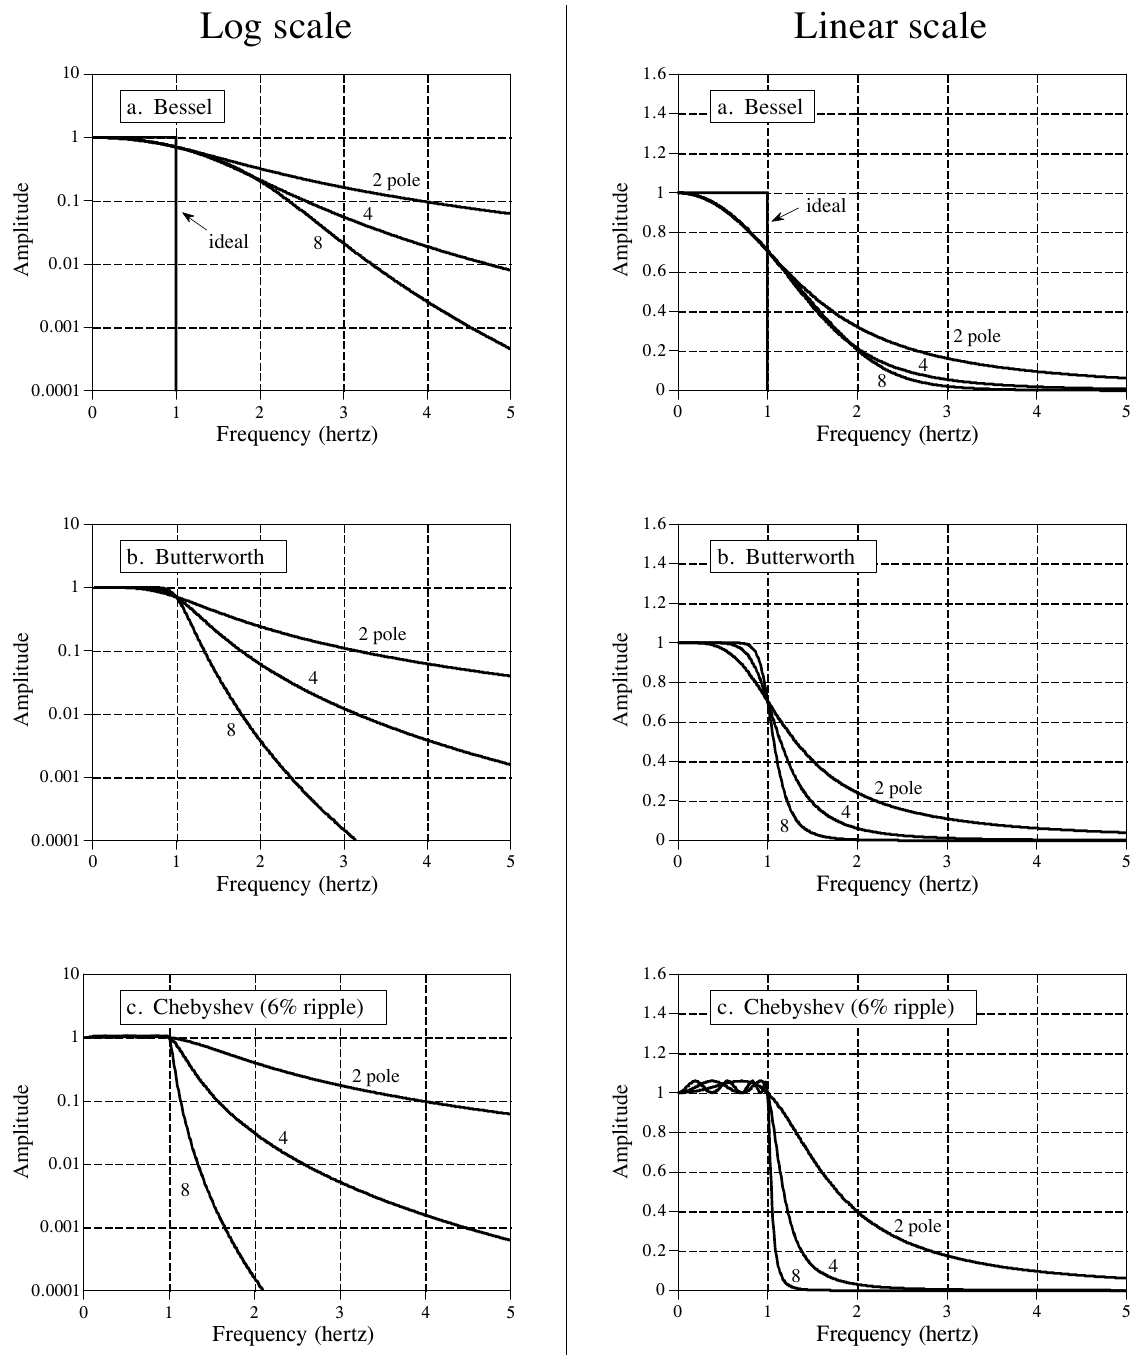
\includegraphics[width=0.950\linewidth,height=0.8\textheight,keepaspectratio]{assets/ch03/fig3-11-12.png}
\caption*{\textbf{图 3-11（左栏）　三种滤波器在对数刻度上的频率响应。}
切比雪夫滤波器的滚降最陡。}
\end{figure}

\textbf{图 3-12（右栏）　三种滤波器在线性刻度上的频率响应。}
巴特沃斯滤波器的通带最平坦。 （Log scale = 对数刻度，Linear scale =
线性刻度。a. 贝塞尔；b. 巴特沃斯；c.~切比雪夫（6\% 纹波）。曲线旁的 2
pole / 4 / 8 = 2/4/8 极点，ideal = 理想响应。Amplitude = 幅度，Frequency
(hertz) = 频率（赫兹）。）

相比之下，巴特沃斯滤波器的优化目标是在通带内不允许纹波的前提下，提供尽可能陡的滚降。它常被称为最大平坦(maximally
flat)滤波器，等同于通带纹波设计为零的切比雪夫滤波器。贝塞尔滤波器在通带内没有纹波，但滚降比巴特沃斯差得多。

最后一个要评估的参数是阶跃响应(step
response)，即输入从一个值迅速变到另一个值时滤波器的反应。图 3-13
是三种滤波器各自的阶跃响应。横轴对应截止频率为 1
赫兹的滤波器，对于更高的截止频率，可以（按反比）换算。例如，截止频率为
1000
赫兹时，阶跃响应的时间单位就是毫秒而不是秒。巴特沃斯和切比雪夫滤波器会出现过冲(overshoot)和振铃(ringing，幅度慢慢衰减的振荡)。相比之下，贝塞尔滤波器没有这两个讨厌的问题。

\begin{figure}[htbp]
\centering
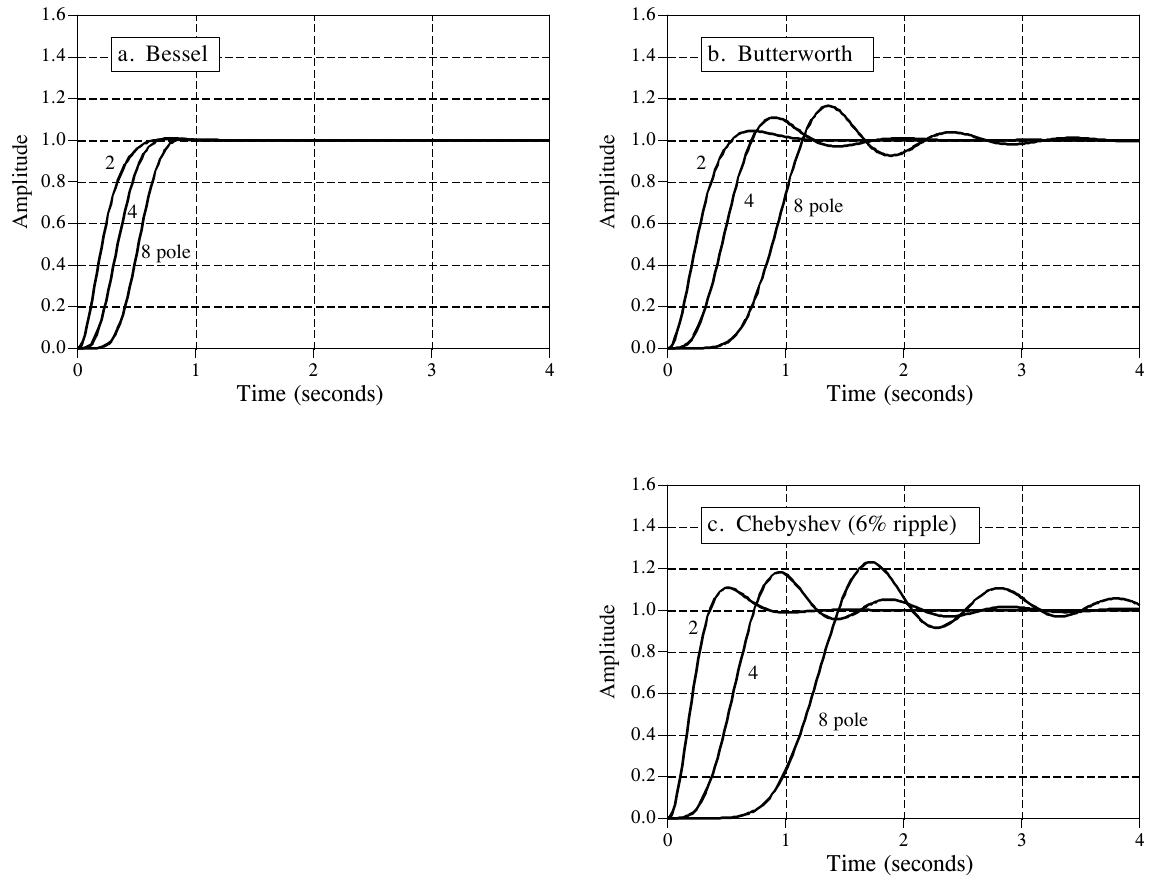
\includegraphics[width=0.971\linewidth,height=0.8\textheight,keepaspectratio]{assets/ch03/fig3-13.png}
\caption*{\textbf{图 3-13　三种滤波器的阶跃响应。} 横轴上的时间对应 1
赫兹的截止频率。在必须把过冲和振铃降到最低时，贝塞尔是最优的滤波器。
（a. 贝塞尔；b. 巴特沃斯；c.~切比雪夫（6\% 纹波）。曲线旁的 2 / 4 / 8
pole = 2/4/8 极点。Amplitude = 幅度，Time (seconds) = 时间（秒）。）}
\end{figure}

图 3-14 进一步说明了贝塞尔滤波器这个非常有利的特性。图 (a)
是一个脉冲波形，可以看作一个上升阶跃接着一个下降阶跃。图 (b) 和 (c)
分别是这个波形经过贝塞尔滤波器和切比雪夫滤波器后的样子。比如说，如果这是一个视频信号，切比雪夫滤波器引入的失真将是灾难性的！过冲会让物体边缘的亮度和中心不一样。更糟的是，物体的左侧会显得亮，右侧会显得暗。许多应用无法容忍阶跃响应表现差。这正是贝塞尔滤波器大显身手的地方：没有过冲，边缘对称。

\begin{figure}[htbp]
\centering
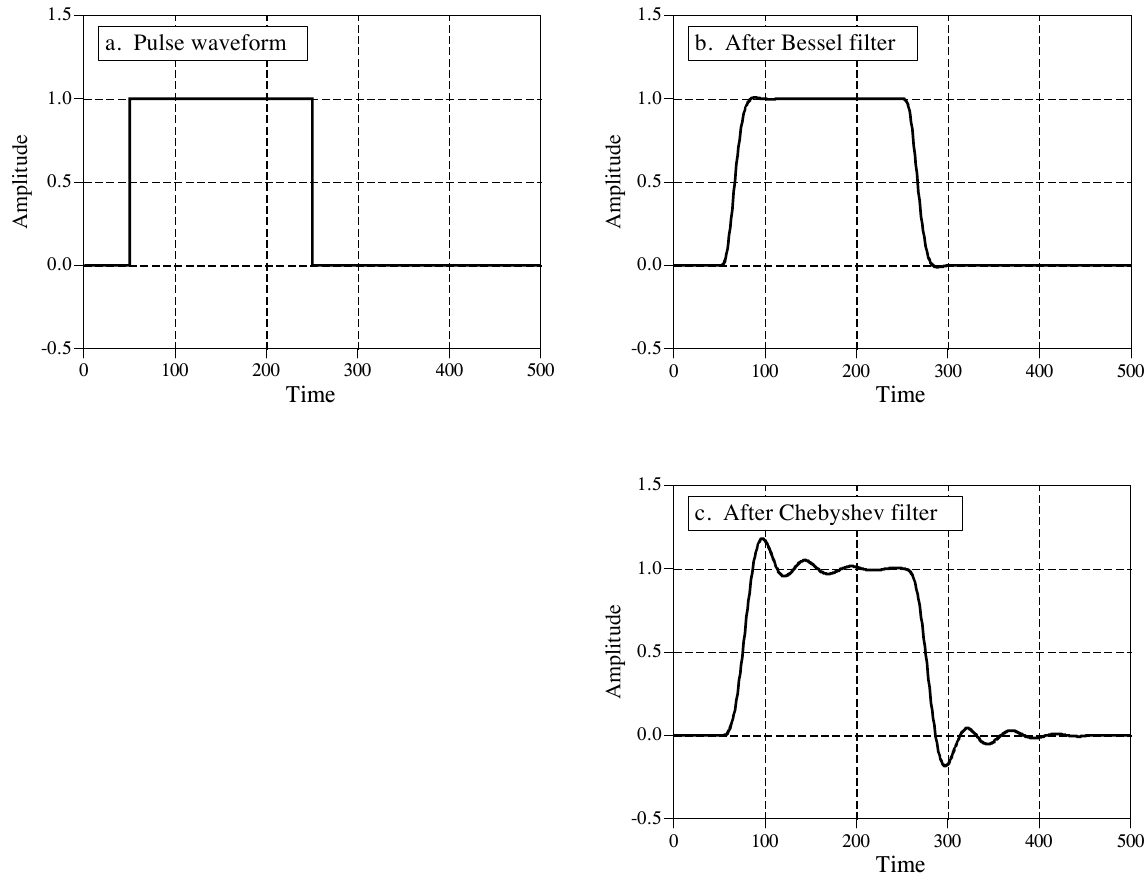
\includegraphics[width=0.954\linewidth,height=0.8\textheight,keepaspectratio]{assets/ch03/fig3-14.png}
\caption*{\textbf{图 3-14　贝塞尔滤波器和切比雪夫滤波器的脉冲响应。}
贝塞尔滤波器的一个关键特性是：滤波器输出中的上升沿和下降沿看起来相似。用这个领域的行话说，这叫线性相位(linear
phase)。图 (b) 是把 (a) 中的脉冲波形通过一个 4
极点贝塞尔滤波器的结果，两个边沿以相似的方式被平滑。图 (c) 是把 (a)
通过一个 4
极点切比雪夫滤波器的结果，左边沿在顶部过冲，右边沿在底部过冲。许多应用不能容忍这种失真。
（a. 脉冲波形(Pulse waveform)；b.
经过贝塞尔滤波器后；c.~经过切比雪夫滤波器后。Amplitude = 幅度，Time =
时间。）}
\end{figure}

\section{如何选择抗混叠滤波器}

表 3-2
总结了这三种滤波器的特性，说明每一种都是以牺牲其他一切为代价来优化某一个参数的：切比雪夫优化滚降，巴特沃斯优化通带平坦度，贝塞尔优化阶跃响应。

\textbf{表 3-2　三种经典滤波器的特性。}
贝塞尔滤波器的阶跃响应最好，因此是时域编码信号的首选。切比雪夫和巴特沃斯滤波器用于消除阻带中的频率，因此非常适合频域编码信号。表中数值的单位是秒和赫兹，对应
1 赫兹的截止频率。

\begingroup\scriptsize\setlength{\tabcolsep}{3pt}

{\def\LTcaptype{none} % do not increment counter
\begin{longtable}[]{@{}
  >{\raggedright\arraybackslash}p{(\linewidth - 16\tabcolsep) * \real{0.0882}}
  >{\raggedright\arraybackslash}p{(\linewidth - 16\tabcolsep) * \real{0.0882}}
  >{\raggedleft\arraybackslash}p{(\linewidth - 16\tabcolsep) * \real{0.1176}}
  >{\raggedleft\arraybackslash}p{(\linewidth - 16\tabcolsep) * \real{0.1176}}
  >{\raggedleft\arraybackslash}p{(\linewidth - 16\tabcolsep) * \real{0.1176}}
  >{\raggedleft\arraybackslash}p{(\linewidth - 16\tabcolsep) * \real{0.1176}}
  >{\raggedleft\arraybackslash}p{(\linewidth - 16\tabcolsep) * \real{0.1176}}
  >{\raggedleft\arraybackslash}p{(\linewidth - 16\tabcolsep) * \real{0.1176}}
  >{\raggedleft\arraybackslash}p{(\linewidth - 16\tabcolsep) * \real{0.1176}}@{}}
\toprule\noalign{}
\begin{minipage}[b]{\linewidth}\raggedright
滤波器
\end{minipage} & \begin{minipage}[b]{\linewidth}\raggedright
极点数
\end{minipage} & \begin{minipage}[b]{\linewidth}\raggedleft
直流电压增益
\end{minipage} & \begin{minipage}[b]{\linewidth}\raggedleft
过冲
\end{minipage} & \begin{minipage}[b]{\linewidth}\raggedleft
稳定到 1\% 的时间
\end{minipage} & \begin{minipage}[b]{\linewidth}\raggedleft
稳定到 0.1\% 的时间
\end{minipage} & \begin{minipage}[b]{\linewidth}\raggedleft
通带纹波
\end{minipage} & \begin{minipage}[b]{\linewidth}\raggedleft
衰减 100 倍的频率
\end{minipage} & \begin{minipage}[b]{\linewidth}\raggedleft
衰减 1000 倍的频率
\end{minipage} \\
\midrule\noalign{}
\endhead
\bottomrule\noalign{}
\endlastfoot
贝塞尔 & 2 & 1.27 & 0.4\% & 0.60 & 1.12 & 0\% & 12.74 & 40.4 \\
& 4 & 1.91 & 0.9\% & 0.66 & 1.20 & 0\% & 4.74 & 8.45 \\
& 6 & 2.87 & 0.7\% & 0.74 & 1.18 & 0\% & 3.65 & 5.43 \\
& 8 & 4.32 & 0.4\% & 0.80 & 1.16 & 0\% & 3.35 & 4.53 \\
巴特沃斯 & 2 & 1.59 & 4.3\% & 1.06 & 1.66 & 0\% & 10.0 & 31.6 \\
& 4 & 2.58 & 10.9\% & 1.68 & 2.74 & 0\% & 3.17 & 5.62 \\
& 6 & 4.21 & 14.3\% & 2.74 & 3.92 & 0\% & 2.16 & 3.17 \\
& 8 & 6.84 & 16.4\% & 3.50 & 5.12 & 0\% & 1.78 & 2.38 \\
切比雪夫 & 2 & 1.84 & 10.8\% & 1.10 & 1.62 & 6\% & 12.33 & 38.9 \\
& 4 & 4.21 & 18.2\% & 3.04 & 5.42 & 6\% & 2.59 & 4.47 \\
& 6 & 10.71 & 21.3\% & 5.86 & 10.4 & 6\% & 1.63 & 2.26 \\
& 8 & 28.58 & 23.0\% & 8.34 & 16.4 & 6\% & 1.34 & 1.66 \\
\end{longtable}
}

\endgroup

（原表把「直流电压增益」到「稳定到 0.1\% 的时间」归为阶跃响应(Step
Response)，后三列归为频率响应(Frequency Response)。）

抗混叠滤波器的选择，几乎完全取决于一个问题：你打算处理的信号是怎样表示信息的。在模拟波形中编码信息的方式有很多，但常见的只有两种：时域编码(time
domain encoding)和频域编码(frequency domain encoding)。这两者的区别在
DSP 中至关重要，也会是贯穿本书的一个反复出现的主题。

在频域编码中，信息包含在组合成信号的那些正弦波里。音频信号就是一个极好的例子。人听语音或音乐时，感知到的声音取决于其中存在哪些频率，而不是波形的具体形状。可以这样证明：让音频信号通过一个电路，这个电路改变各个正弦波的相位，但保留它们的频率和幅度。得到的信号在示波器上看起来完全不同，听起来却一模一样。尽管波形被大大改变了，有用的信息却完好无损。由于混叠会把频率成分放错位置并让它们重叠，它会直接破坏在频域中编码的信息。因此，这类信号的数字化通常要配一个截止陡峭的抗混叠滤波器，比如切比雪夫、椭圆或巴特沃斯滤波器。那这些滤波器糟糕的阶跃响应怎么办？无所谓，编码的信息不受这种失真的影响。

相反，时域编码用波形的形状来存储信息。例如，医生可以在病人的胸部和手臂上贴电极（心电图，electrocardiogram，简称
EKG），监测心脏的电活动。EKG
波形的形状提供了所需的信息，比如心跳过程中各个心腔在什么时候收缩。图像是这类信号的另一个例子。图像不是随时间变化的波形，而是把信息编码在随距离变化的波形形状中。图片由一块块亮度和颜色区域构成，以及它们和其他亮度、颜色区域之间的关系。你看《蒙娜丽莎》时不会说：「哇，好一组有趣的正弦波。」

问题就在这里：采样定理分析的是数字化过程中频域里发生了什么。这让它非常适合用来理解那些信息编码在频域中的信号的模数转换。然而，对于理解时域编码信号应该怎样数字化，采样定理帮不上什么忙。我们来仔细看看。

图 3-15 说明了数字化时域编码信号的几种选择。图 (a)
是一个待数字化的模拟信号示例。这里我们想捕获的信息是矩形脉冲的形状。这个示例信号中还包含一小段高频正弦波的猝发(burst)，它代表模拟信号上总会出现的宽带噪声、干扰之类的垃圾。其他几幅图显示了在不同抗混叠滤波器选项下数字化信号的样子：切比雪夫滤波器、贝塞尔滤波器，以及不用滤波器。

重要的是要明白，这些选项都无法让原始信号从采样数据中重建出来。这是因为原始信号本身就包含高于采样率一半的频率成分。既然这些频率不可能存在于数字化信号中，重建出来的信号也就不可能包含它们。这些高频有两个来源：(1)
噪声和干扰，这是你想消除的；(2)
波形中的陡峭边沿，其中很可能包含你想保留的信息。

\begin{enumerate}
\def\labelenumi{(\alph{enumi})}
\setcounter{enumi}{1}
\item
  中的切比雪夫滤波器解决问题的方式，是大刀阔斧地去掉所有高频成分。这样得到的滤波后模拟信号可以被采样，之后再完美重建。然而，重建出的模拟信号和滤波后的信号相同，而不是和原始信号相同。虽然采样过程中没有丢失任何东西，但波形已经被抗混叠滤波器严重扭曲了。如
  (b) 所示，这药方比病本身还糟！别这么干！
\item
  中的贝塞尔滤波器正是为这个问题设计的。它的输出和原始波形非常相似，只是边沿被温和地磨圆了。调整滤波器的截止频率，可以在边沿的平滑程度和消除信号中高频成分之间做取舍。滤波器用更多的极点，能在这两个参数之间取得更好的平衡。一条常用的经验法则是把截止频率设为采样频率的大约四分之一。这样每个边沿的上升段上大约有两个采样。注意贝塞尔和切比雪夫滤波器都去掉了原始信号中的那段高频噪声猝发。
\end{enumerate}

最后一种选择是完全不用抗混叠滤波器，如 (d)
所示。它有一个很大的优点：每个采样的值都和原始模拟信号的值相同。换句话说，它的边沿锐度是完美的：原始信号的变化会立即反映在数字数据中。缺点是混叠会扭曲信号。这有两种不同的表现形式。第一，高频干扰和噪声（比如示例中的正弦猝发）会变成毫无意义的采样，如
(d)
所示。也就是说，模拟信号中的任何高频噪声，都会以混叠噪声的形式出现在数字信号中。从更一般的意义上说，这不是采样的问题，而是上游模拟电路的问题。降低噪声和干扰不是
ADC
的职责，而是数字化之前的模拟电路的责任。结果可能是应该在数字化器之前放一个贝塞尔滤波器来控制这个问题。但这意味着这个滤波器应被视为模拟处理的一部分，而不是为了数字化器而做的事。

混叠的第二种表现更微妙。当模拟信号中发生某个事件（比如一个边沿）时，(d)
中的数字信号要到下一个采样才能察觉这个变化。数字数据中没有任何信息表明两个采样之间发生了什么。现在，就这个问题比较一下不用滤波器和用贝塞尔滤波器。例如，设想在
(c)
的采样之间画直线。这条构造出来的直线穿过阶跃幅度一半的那个时刻，就给出了模拟信号中边沿发生时刻的亚采样(subsample)估计。不用滤波器时，这种亚采样信息就完全丢失了。要评估这对你的具体情况有什么影响，用不着什么高深的定理，只需要清楚地知道数据采集到之后你打算拿它做什么。

\section{多速率数据转换}

电子学中有一股用数字算法取代模拟电路的强劲趋势，数据转换就是一个极好的例子。考虑设计一个数字录音机：这个系统要把语音信号数字化，以数字形式存储数据，之后再重建信号用于回放。要再现可懂的语音，系统必须捕获大约
100 到 3000
赫兹之间的频率。然而，麦克风产生的模拟信号还包含高得多的频率，比如高达
40 kHz。蛮力做法是让模拟信号通过一个截止频率为 3 kHz 的 8
极点低通切比雪夫滤波器，再以 8 kHz 采样。在另一端，DAC 用零阶保持以 8
kHz 重建模拟信号，再用另一个 3 kHz 的切比雪夫滤波器得到最终的语音信号。

\begin{figure}[htbp]
\centering
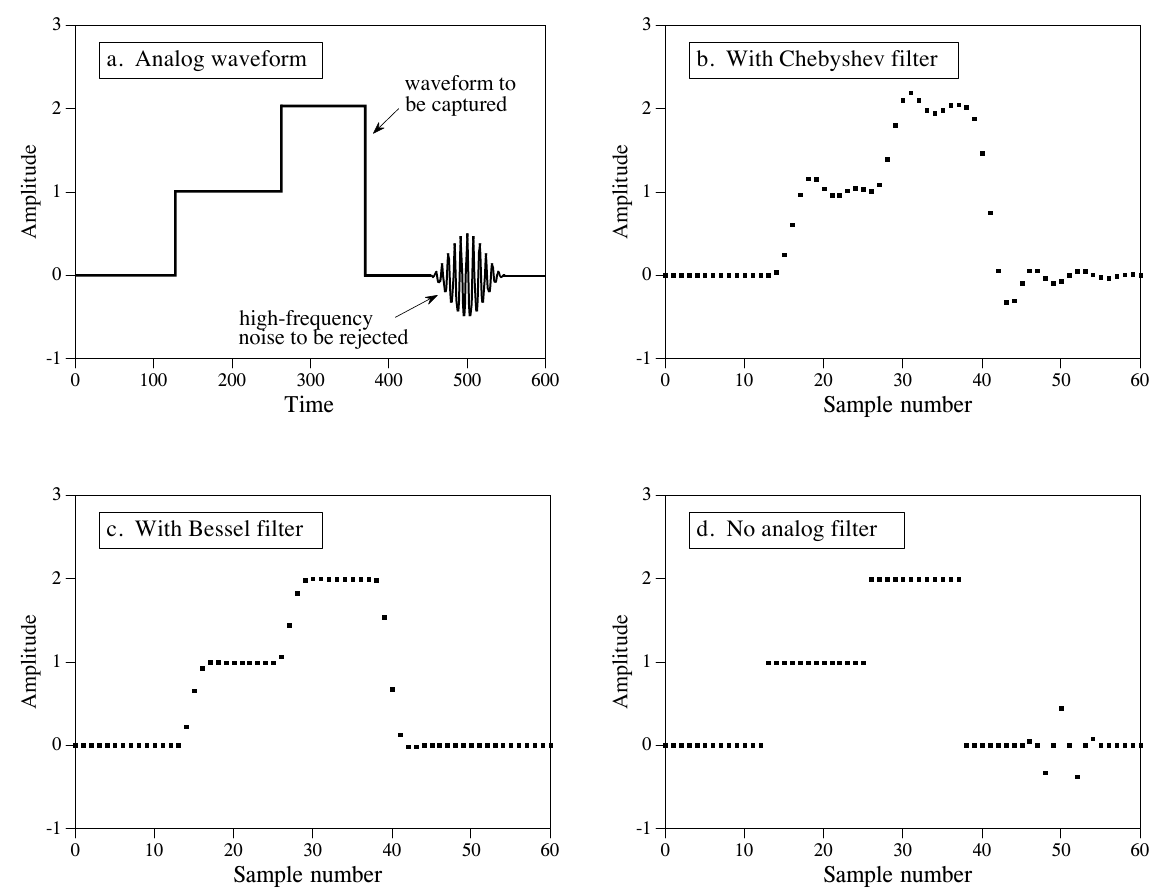
\includegraphics[width=0.967\linewidth,height=0.8\textheight,keepaspectratio]{assets/ch03/fig3-15.png}
\caption*{\textbf{图 3-15　时域编码信号的三种抗混叠滤波方案。}
目标是消除（采样时会混叠的）高频，同时保留（承载信息的）边沿锐度。图 (a)
是一个既有陡峭边沿、又有一段高频噪声猝发的模拟信号示例。图 (b)
是用切比雪夫滤波器得到的数字化信号。高频虽然被有效去除了，边沿却被严重扭曲。这通常是个糟糕的方案。(c)
中的贝塞尔滤波器在去除高频的同时，只对边沿做了温和的平滑。图 (d)
是不用抗混叠滤波器得到的数字化信号。这时边沿保持了完美的锐度，但高频猝发混叠成了几个毫无意义的采样。
（a. 模拟波形(Analog waveform)，waveform to be captured =
要捕获的波形，high-frequency noise to be rejected = 要滤除的高频噪声；b.
用切比雪夫滤波器；c.~用贝塞尔滤波器；d.~不用模拟滤波器。Amplitude =
幅度，Time = 时间，Sample number = 采样序号。）}
\end{figure}

以比这种直接分析更快的速率采样，有许多实用的好处。例如，设想用 64 kHz
的采样率重新设计这个数字录音机。抗混叠滤波器的任务变容易了：让 3 kHz
以下的所有频率通过，同时阻断 32 kHz
以上的所有频率。重建滤波器也有类似的简化。简而言之，更高的采样率让 8
极点滤波器可以换成简单的电阻-电容（RC）网络。问题在于，数字系统现在被更高采样率带来的数据淹没了。

更进一步的做法是多速率技术，即在同一个系统中使用不止一种采样率。以数字录音机为例，它是这样工作的。第一，让语音信号通过一个简单的
RC 低通滤波器，以 64 kHz 采样。得到的数字数据包含所需的 100 到 3000
赫兹语音频带，也包含 3 kHz 到 32 kHz
之间不可用的频带。第二，在软件中用一个 3 kHz
的数字低通滤波器去掉这些不可用的频率。第三，把数字信号从 64 kHz 重采样到
8 kHz，做法就是每 8 个采样丢掉 7
个，这个过程叫抽取(decimation)。得到的数字数据，等同于用激进的模拟滤波加上直接
8 kHz 采样所得到的数据。

多速率技术也可以用在这个示例系统的输出部分。从存储器中取出 8 kHz
的数据，把它转换成 64 kHz
的采样率，这个过程叫插值(interpolation)。做法是在从存储器取出的每两个采样之间插入七个值为零的采样。得到的信号是一个数字冲激串，包含所需的
100 到 3000 赫兹语音频带，以及 3 kHz 到 32 kHz 之间的频谱复制。回头看图
3-6 的 (a) 和 (b) 就能明白为什么会这样。然后用一个数字低通滤波器去掉 3
kHz 以上的一切。经 DAC 转换成模拟信号后，只需要一个简单的 RC
网络就能得到最终的语音信号。

多速率数据转换的价值有两点：(1)
它用软件取代了模拟元件，这在大批量生产的产品中有明显的经济优势；(2)
它能在关键应用中达到更高的性能水平。例如，CD
音频系统就用这类技术获得尽可能好的音质。性能的提升来自用数字算法（舍入误差带来的精度为
0.0001\%）取代模拟元件（精度
1\%）。后面的章节会讲到，数字滤波器在一些关键方面比模拟滤波器强几百倍。

\section{单比特数据转换}

单比特 ADC 和 DAC
是电信和高保真音乐重放中一种流行的技术。它们属于多速率技术，用更高的采样率换取更少的比特数。极端情况下，每个采样只需要一个比特。电路结构虽然多种多样，但大多基于增量调制(delta
modulation)。下面介绍三个示例电路，让你对这个领域有个大致的感觉。这些电路都做在集成电路里，所以不用操心每个晶体管和运放该放在哪里。没人会要你用基本元件搭一个这样的电路。

图 3-16
是一个典型增量调制器的框图。模拟输入是一个幅度为几伏的语音信号，输出信号是一串数字
1 和
0。比较器(comparator)判断进入的模拟信号和电容上存储的电压哪个更高。这个判断以数字
1 或 0
的形式送到锁存器(latch)的输入端。在每个时钟脉冲（通常是几百千赫兹）到来时，锁存器把输入端出现的数字状态传到输出端。这个锁存器保证输出与时钟同步，从而确定了采样率，即
1 比特输出能够更新自己的速率。

\begin{figure}[htbp]
\centering
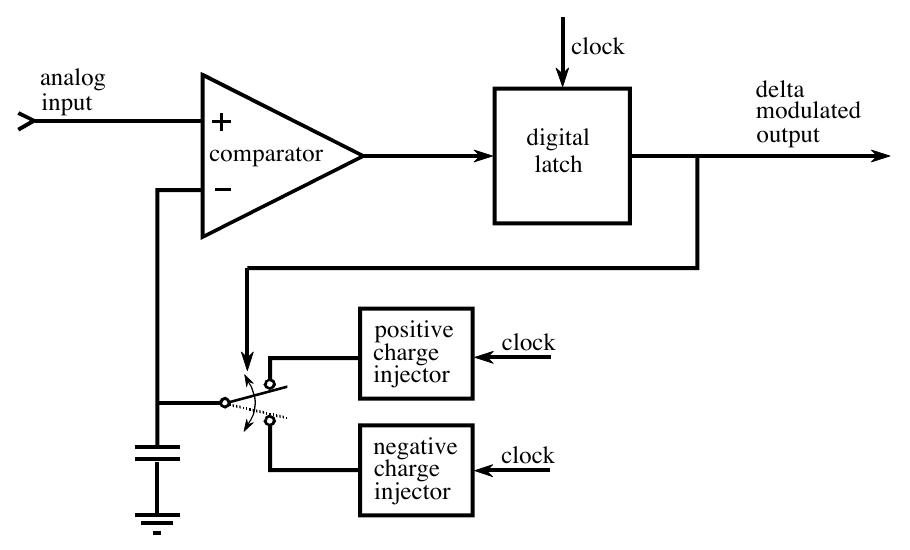
\includegraphics[width=0.758\linewidth,height=0.8\textheight,keepaspectratio]{assets/ch03/fig3-16.png}
\caption*{\textbf{图 3-16　增量调制电路框图。}
输入电压与电容上存储的电压比较，结果以数字 0 或 1
送到锁存器的输入端。锁存器的输出与时钟同步更新，并用在一个反馈回路中，使电容电压跟踪输入电压。
（analog input = 模拟输入，comparator = 比较器，latch = 锁存器，clock =
时钟，delta modulated digital output = 增量调制的数字输出，positive /
negative charge injector = 正/负电荷注入器。）}
\end{figure}

把数字输出拿来驱动一个电子开关，就形成了反馈回路。如果输出是数字
1，开关把电容接到正电荷注入器(positive charge
injector)。这是一个很宽泛的说法，指的是每个时钟周期把电容上的电压提高一个固定量（比如
1 毫伏）的电路。它可能只是一个接到较高正电压的电阻。如果输出是数字
0，开关接到负电荷注入器，它把电容上的电压降低同样的固定量。

图 3-17
说明了这个电路产生的信号。在时间为零时，模拟输入和电容上的电压都从零开始。如
(a) 所示，输入信号在第八个时钟周期突然升到 9.5
伏。由于输入信号现在比电容上的电压更正，数字输出变为 1，如 (b)
所示。这使开关接到正电荷注入器，电容上的电压在每个时钟周期增加一小步。虽然
(a) 中画的是每个时钟周期增加 1 伏，但这只是为了示意，更典型的值是 1
毫伏。电容电压的这种阶梯式上升一直持续到它超过输入信号的电压为止。此时系统达到平衡，输出在数字
1 和 0 之间振荡，使电容上的电压在 9 伏和 10
伏之间振荡。就这样，电路的反馈迫使电容电压跟踪输入信号的电压。如果输入信号变化得非常快，电容上的电压会以恒定的速率变化，直到追上为止。这个恒定的变化率叫压摆率(slew
rate)，和运放等其他电子器件中的叫法一样。

现在来看增量调制输出信号的特性。如果模拟输入的值在增加，输出信号中 1
会比 0 多。同样，如果模拟输入的值在减小，输出中 0 会比 1
多。如果模拟输入恒定，数字输出会在 0 和 1
之间交替，两者个数相等。说得更一般些，1 和 0
的相对数量与模拟输入的斜率（导数(derivative)）成正比。

\begin{figure}[htbp]
\centering
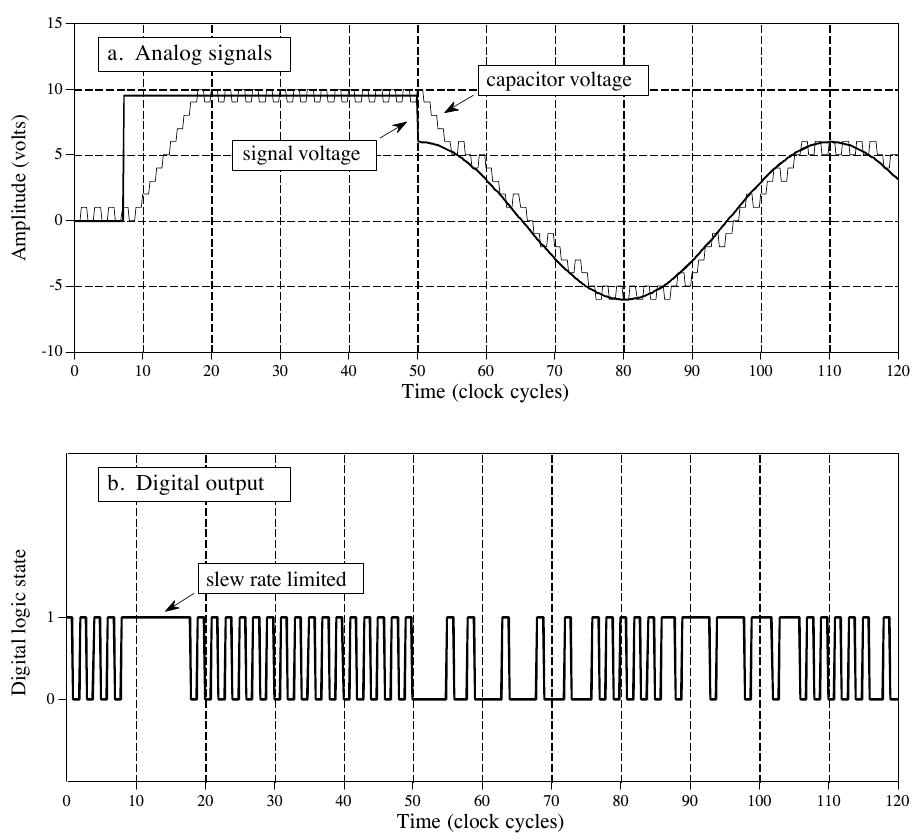
\includegraphics[width=0.767\linewidth,height=0.8\textheight,keepaspectratio]{assets/ch03/fig3-17.png}
\caption*{\textbf{图 3-17　图 3-16 中增量调制器产生的信号示例。} 图 (a)
是模拟输入信号以及电容上对应的电压。图 (b) 是增量调制的输出，即一串数字
1 和 0。 （a. 模拟信号(Analog signals)：capacitor voltage =
电容电压，signal voltage = 信号电压，Amplitude (volts) = 幅度（伏）；b.
数字输出(Digital output)：Digital logic state = 数字逻辑状态，slew rate
limited = 受压摆率限制。Time (clock cycles) = 时间（时钟周期）。）}
\end{figure}

这个电路是把模拟信号转换成一串串行的 1 和
0、用于传输或数字存储的廉价方法。一个特别吸引人的特点是：所有比特的含义都相同，不像传统的串行格式那样分为起始位、LSB、\ldots、MSB、停止位。接收端的电路和发送电路的反馈部分完全相同。正如发送电路中电容上的电压跟随模拟输入一样，接收电路中电容上的电压也是如此。也就是说，(a)
中的电容电压也代表了重建信号的样子。

这个电路的一个关键局限，是 (1) 最大压摆率、(2) 量化步长和 (3)
数据率三者之间不可避免的权衡。具体来说，如果把最大压摆率和量化步长调到语音通信可以接受的值，数据率最终会落在
MHz 量级。这太高了，没有商业价值。例如，常规的语音信号采样只需要每秒约
64,000 比特。

图 3-18 给出了这个问题的一个解决方案：连续可变斜率增量(CVSD,
Continuously Variable Slope Delta)调制器，摩托罗拉 MC3518
系列实现了这一技术。这种方法把时钟速率和量化步长设成可以接受的值，比如
30 kHz 和 2000
级。这会导致压摆率非常差，于是用附加电路来校正。工作时，一个移位寄存器(shift
register)持续观察系统最近产生的四个比特。如果电路处于受压摆率限制的状态，最近四个比特就会全是
1（正斜率）或全是
0（负斜率）。一个逻辑电路检测到这种情况，产生一个模拟信号，提高电荷注入器产生的电荷量。这通过增大加到电容上的电压步长来提高压摆率。

逻辑电路和电荷注入器之间通常会放一个模拟滤波器。这让步长取决于电路已经处于压摆受限状态多长时间。只要电路一直压摆受限，步长就会越来越大。这常被称为音节滤波器(syllabic
filter)，因为它的特性取决于构成语音的音节的平均长度。经过适当的优化（来自芯片厂商的规格书，而不是你自己的工作），16
到 32 kHz
的数据率就能产生质量可接受的语音。不断变化的步长让数字数据很难看懂，但幸运的是，你也不需要看懂。在接收端，用一个和发送电路中完全相同的音节滤波器来重建模拟信号。如果两个滤波器匹配，CVSD
调制带来的失真就很小。CVSD 可能是以数字方式传输语音信号最简单的方法。

\begin{figure}[htbp]
\centering
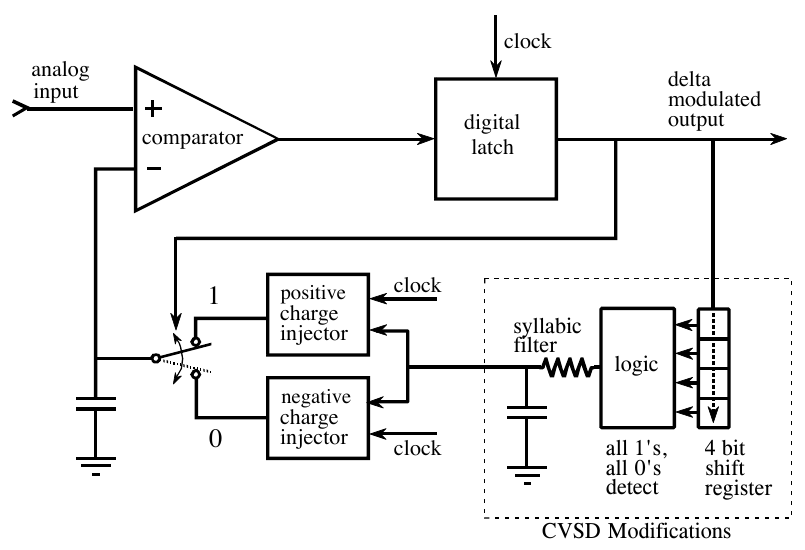
\includegraphics[width=0.671\linewidth,height=0.8\textheight,keepaspectratio]{assets/ch03/fig3-18.png}
\caption*{\textbf{图 3-18　CVSD 调制框图。}
在基本的增量调制器上加了一个逻辑电路，以改善压摆率。 （在图 3-16
的基础上新增「CVSD Modifications = CVSD 改动」部分：4 bit shift register
= 4 比特移位寄存器，all 1's, all 0's detect = 全 1/全 0 检测，logic =
逻辑电路，syllabic filter = 音节滤波器。）}
\end{figure}

CVSD
调制虽然非常适合编码语音信号，却不能用于通用的模数转换。即使你能绕开「数字数据与输入信号的导数相关」这一点，变化的步长也会把事情搞得无法收拾。此外，模拟信号的直流电平通常不会被数字数据捕获。

图 3-19 所示的增量-累加转换器(delta-sigma converter)，巧妙地把模拟电路和
DSP
算法结合起来，消除了这些问题。注意电容上的电压现在是和地电位比较。反馈回路也做了修改：电路输出数字
1 时，电容上的电压降低；输出数字 0
时，电压升高。当输入信号的电压升高和降低时，它会试图抬高和压低电容上的电压。比较器检测到这种电压变化，于是电荷注入器产生抵消的电荷，使电容保持在零伏。

如果输入电压为正，数字输出中 1 会比 0 多，多出来的 1
用来产生负电荷，与正的输入信号抵消。同样，如果输入电压为负，数字输出中 0
会比 1 多，提供净的正电荷注入。如果输入信号等于零伏，输出中 1 和 0
的个数相等，总的电荷注入为零。

现在，输出中 1 和 0
的相对数量与输入电压的电平相关，而不是像前一个电路那样与斜率相关。这就简单多了。例如，把数字输出送进一个计数器，统计
4096 个时钟周期里 1 的个数，就构成了一个 12 比特 ADC。数字 4095
对应最大的正输入电压，数字 0 对应最大的负输入电压，2048
对应零输入电压。这也说明了「增量-累加(delta-sigma)」这个名字的由来：先做增量调制(delta)，再做求和(sigma)。

\begin{figure}[htbp]
\centering
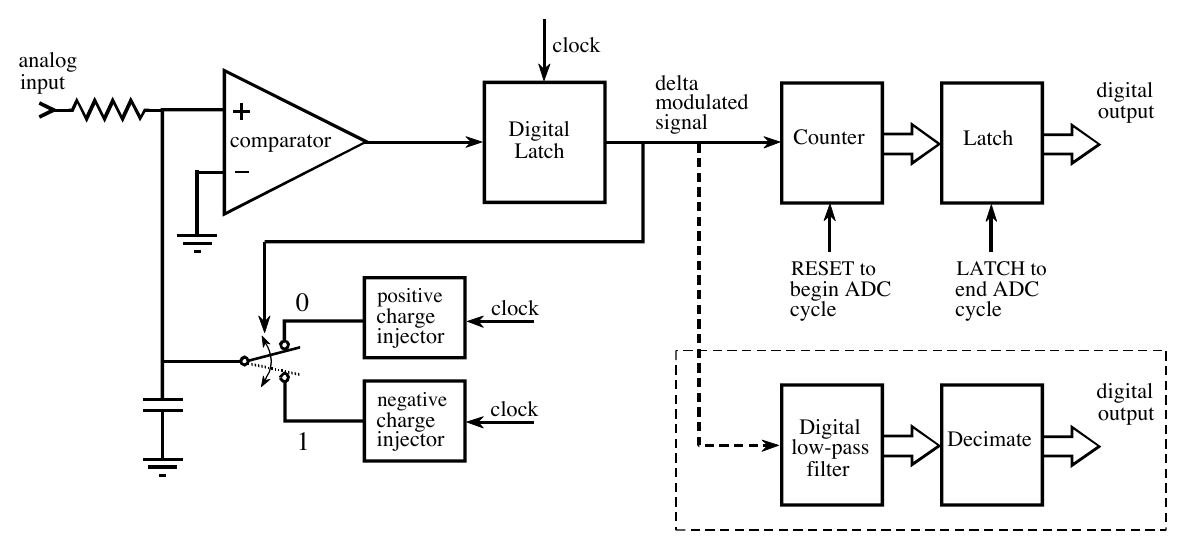
\includegraphics[width=0.983\linewidth,height=0.8\textheight,keepaspectratio]{assets/ch03/fig3-19.png}
\caption*{\textbf{图 3-19　增量-累加模数转换器框图。}
最简单的情况下，对增量调制器输出的脉冲计数，计满预定的时钟周期数，然后锁存计数器的输出，完成一次转换。在更复杂的电路中，脉冲先经过一个数字低通滤波器，再重采样（抽取）到较低的采样率。
（delta modulated signal = 增量调制信号，Digital Counter =
数字计数器，Latch = 锁存器，RESET to begin ADC cycle = 复位以开始一次
ADC 周期，LATCH to end ADC cycle = 锁存以结束一次 ADC 周期，Digital
low-pass filter = 数字低通滤波器，Decimate = 抽取，digital output =
数字输出。）}
\end{figure}

这类增量调制器产生的 1 和
0，很容易变回模拟信号。只需要一个模拟低通滤波器，可能简单到只是一个 RC
网络。数字 1 和 0
对应的高低电压平均下来，就形成正确的模拟电压。例如，假设 1 和 0 分别用 5
伏和 0 伏表示。如果数据流中 80\% 的比特是 1、20\% 是
0，低通滤波器的输出就是 4 伏。

这种把单比特数据流变回原始波形的方法，因为几个原因而很重要。第一，它提供了一种取代增量-累加
ADC
电路中计数器的巧妙办法：不再简单地对增量调制器输出的脉冲计数，而是让这个二值信号通过一个数字低通滤波器，再抽取以降低采样率。例如，这个过程可能先把数字流中的每个
1 和 0 变成一个 12 比特的采样：1 变成 4095，0 变成
0。对这个信号做数字低通滤波，就得到原始波形的数字化版本，正如模拟低通滤波器会得到模拟复现一样。然后抽取丢掉大部分采样，降低采样率。结果得到的数字信号，等同于对原始波形直接采样。

许多商用 ADC
用这种方法数字化语音和其他音频信号。一个例子是美国国家半导体(National
Semiconductor)的 ADC16071，它能以最高 192 kHz 的采样率做 16
比特模数转换。采样率为 100 kHz 时，增量调制器的时钟频率为 6.4
MHz。数字低通滤波器是一个 246 点的 FIR 滤波器，第 16
章会介绍这种滤波器。它去掉数字数据中 50
kHz（最终采样率的一半）以上的所有频率。从概念上说，可以把它看作形成了一个
6.4 MHz、每个采样 16 比特的数字信号。然后把信号从 6.4 MHz 抽取到 100
kHz，做法是每 64 个采样删掉 63
个。实际工作中，这个器件内部发生的事情比这段简单讨论描述的要多得多。

增量-累加转换器也可以用于语音和音频信号的数模转换。从存储器中取出数字信号，把它转换成增量调制的
1 和 0
流。如上所述，用一个简单的模拟低通滤波器，就能很容易地把这个单比特信号变成重建的模拟信号。和抗混叠滤波器一样，通常只需要一个
RC 网络。这是因为大部分滤波工作都由高性能的数字滤波器完成了。

增量-累加 ADC
有几个怪癖，限制了它们只能用于特定的应用。例如，很难对它们的输入做多路复用(multiplex)。当输入从一个信号切换到另一个信号时，要等数字滤波器把前一个信号的数据清空之后，才能恢复正常工作。增量-累加转换器在另一方面也有局限：你不知道每个采样确切是在什么时刻取的。每个采到的采样，都是在输入信号的一段区间上取得的
1
比特信息的综合。对于音频这类频域编码的信号，这不是问题；但对于时域编码的信号，这是一个重大的局限。要理解信号波形的形状，你常常需要知道每个采样被取的精确时刻。最后，这些器件大多是专门为音频应用设计的，它们的性能指标也是相应地给出的。例如，一个用于语音信号的
16 比特 ADC，并不一定意味着每个采样都有 16
比特的精密度。更可能的是，厂商的意思是语音信号可以被数字化到 16
比特的动态范围(dynamic
range)。别指望在通用数据采集中从这种器件得到完整的 16 比特有用信息。

这些解释和例子虽然介绍了单比特 ADC 和 DAC，但必须强调，它们只是对复杂的
DSP
和集成电路技术的简化描述。你不会指望厂商把芯片的全部内部工作原理告诉竞争对手，所以也别指望他们会告诉你。
